\subsubsection{EVEN y ODD} \label{sssec:skipp}

En las Figs. \ref{fig:Hval_Even} y \ref{fig:Hval_Odd} podemos ver que los cuantificadores relacionados con el histograma de valores normalizado se degradan ligeramente con el procedimiento skipping.
Por ejemplo, $\left \langle H_{hist} \right \rangle$ reduce de $0.9722$ sin saltarse a $0.9459$ para EVEN y $0.9706$ para ODD.
Esta diferencia entre EVEN y ODD en coma flotante se debe a que se obtuvo una alta dispersión para $H_{hist}$, $H_{BP}$ y $C_{BP}$ pero no para $H_{BPW}$ o $C_{BPW}$.

Las figuras \ref{fig:Hbp_Even} a \ref{fig:MP_Even} y las Figs. \ref{fig:Hbp_Odd} a \ref{fig:MP_Odd} muestran los resultados de los cuantificadores BP y BPW para EVEN y ODD, respectivamente.
Se requiere una mayor precisión para lograr una complejidad menor, a diferencia de los casos sin skipping que convergen a valores altos.
Desde el punto de vista de MP, se obtiene una gran mejora utilizando cualquiera de las estrategias de omisión, pero el ODD es ligeramente mejor que EVEN.
Los patrones faltantes se reducen a $MP = 118$ para EVEN y ODD, lo que aumenta la entropía Bandt \& Pompe máxima permitida que alcanza el valor medio $\left \langle H_{BP} \right \rangle = 0.8381$ para EVEN, y $ \left \langle H_{BP} \right \rangle = 0.9094$.
La complejidad se reduce a $\left \langle C_{BP} \right \rangle = 0.224$ para EVEN y $\left \langle C_{BP} \right \rangle = 0.282$ para ODD.
El número mínimo de bits para converger a este valor es de $ B> 40 $ para los mapas EVEN y ODD.
%
\begin{figure}[htpb]
	\centering
	\begin{subfigure}[b]{0.49\textwidth}
		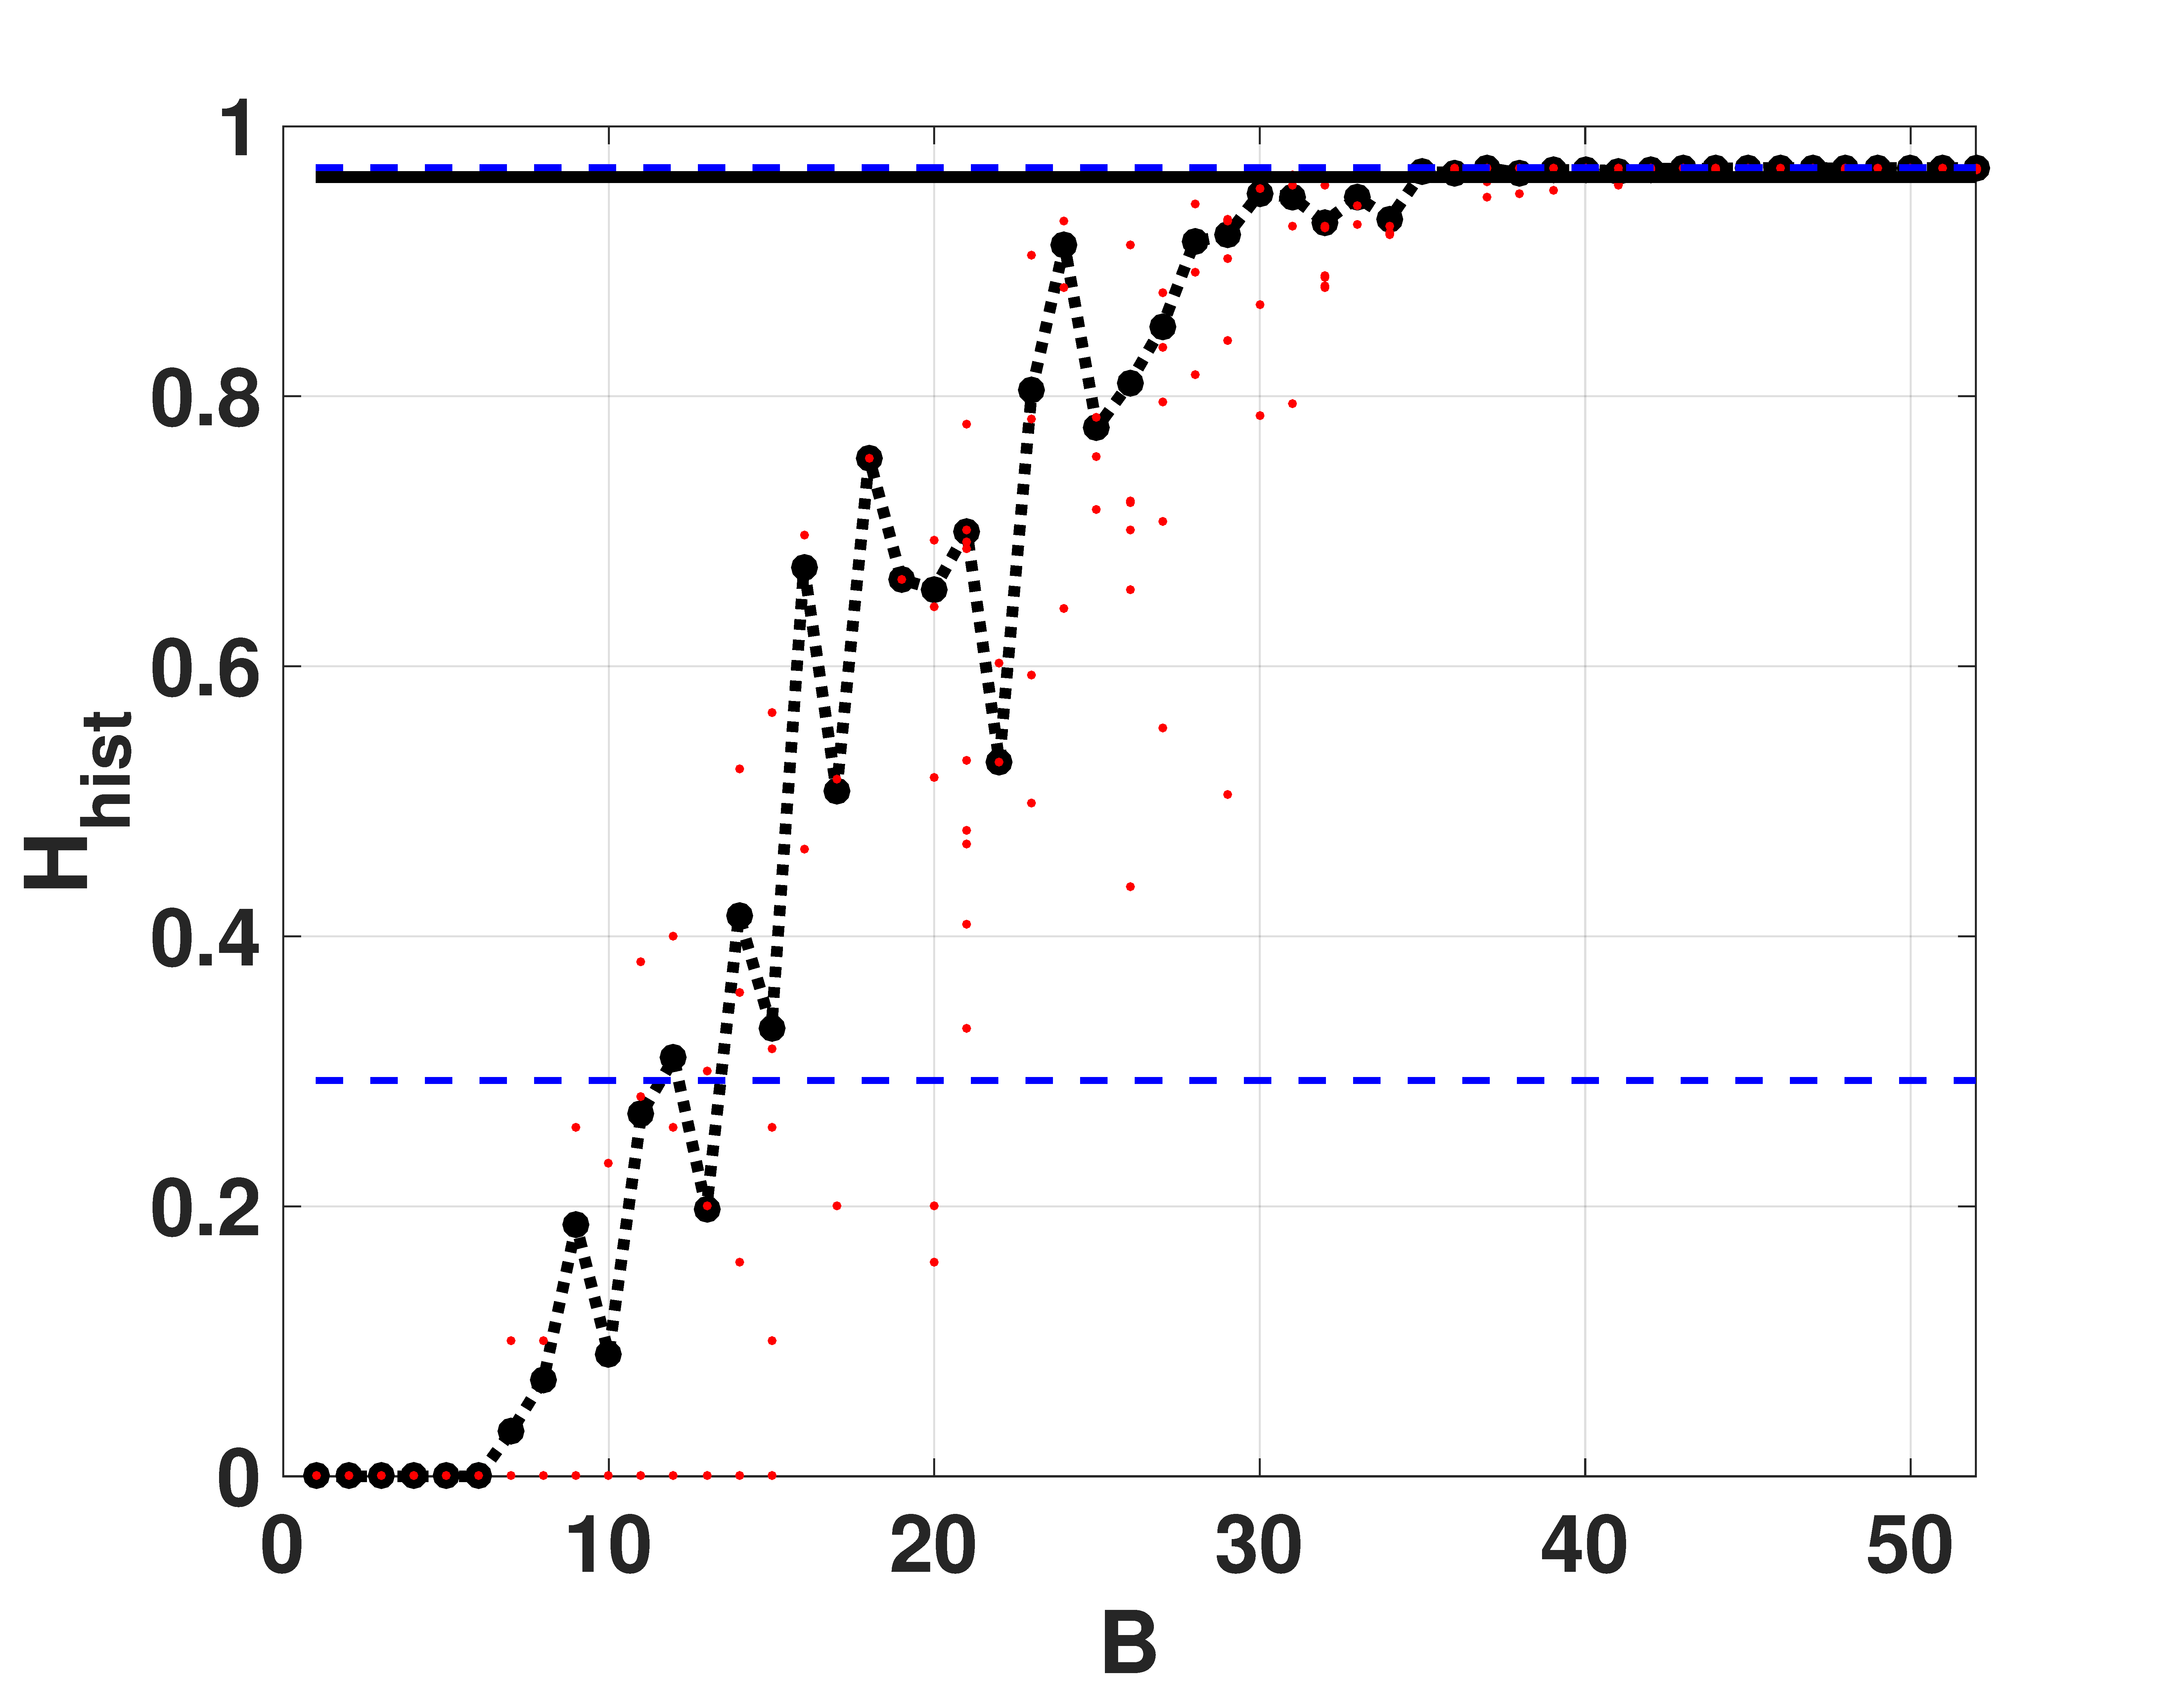
\includegraphics[width=\textwidth]{Hval_Even}
		\caption{$H_{hist}$ vs. $B$}
		\label{fig:Hval_Even}
	\end{subfigure}
	\begin{subfigure}[b]{0.49\textwidth}
		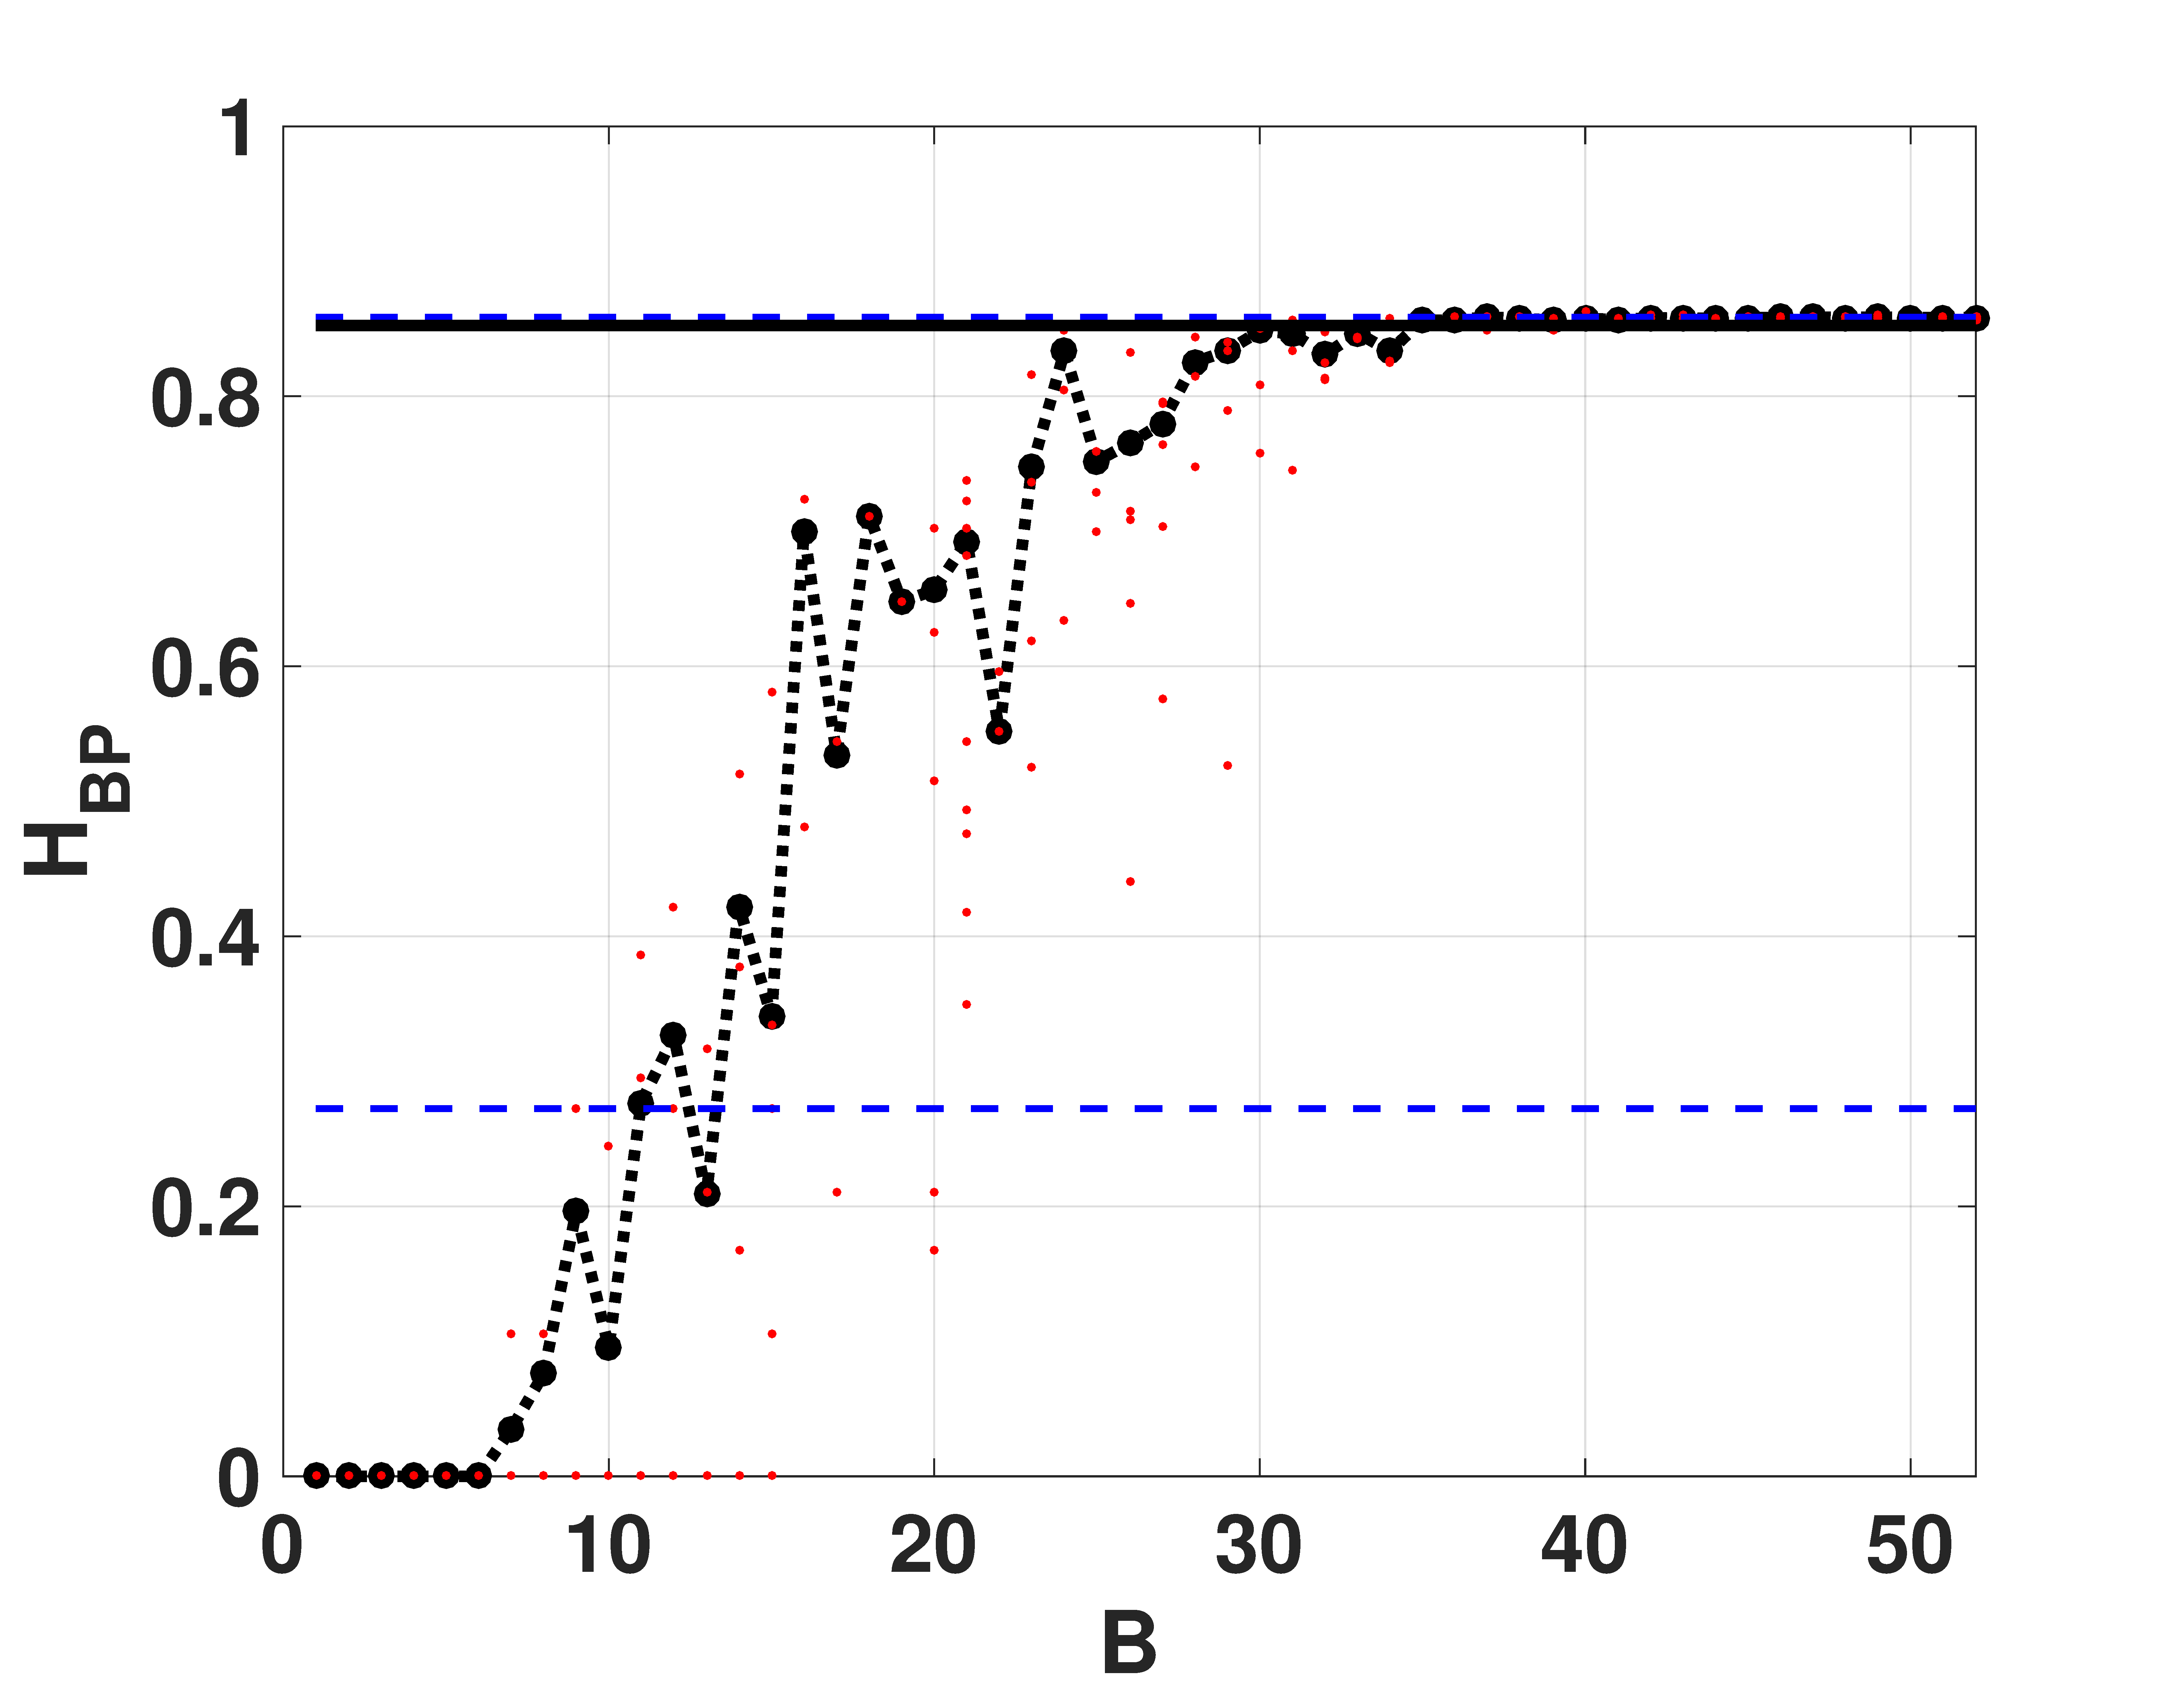
\includegraphics[width=\textwidth]{Hbp_Even}
		\caption{$H_{BP}$ vs. $B$}
		\label{fig:Hbp_Even}
	\end{subfigure}
	\begin{subfigure}[b]{0.49\textwidth}
		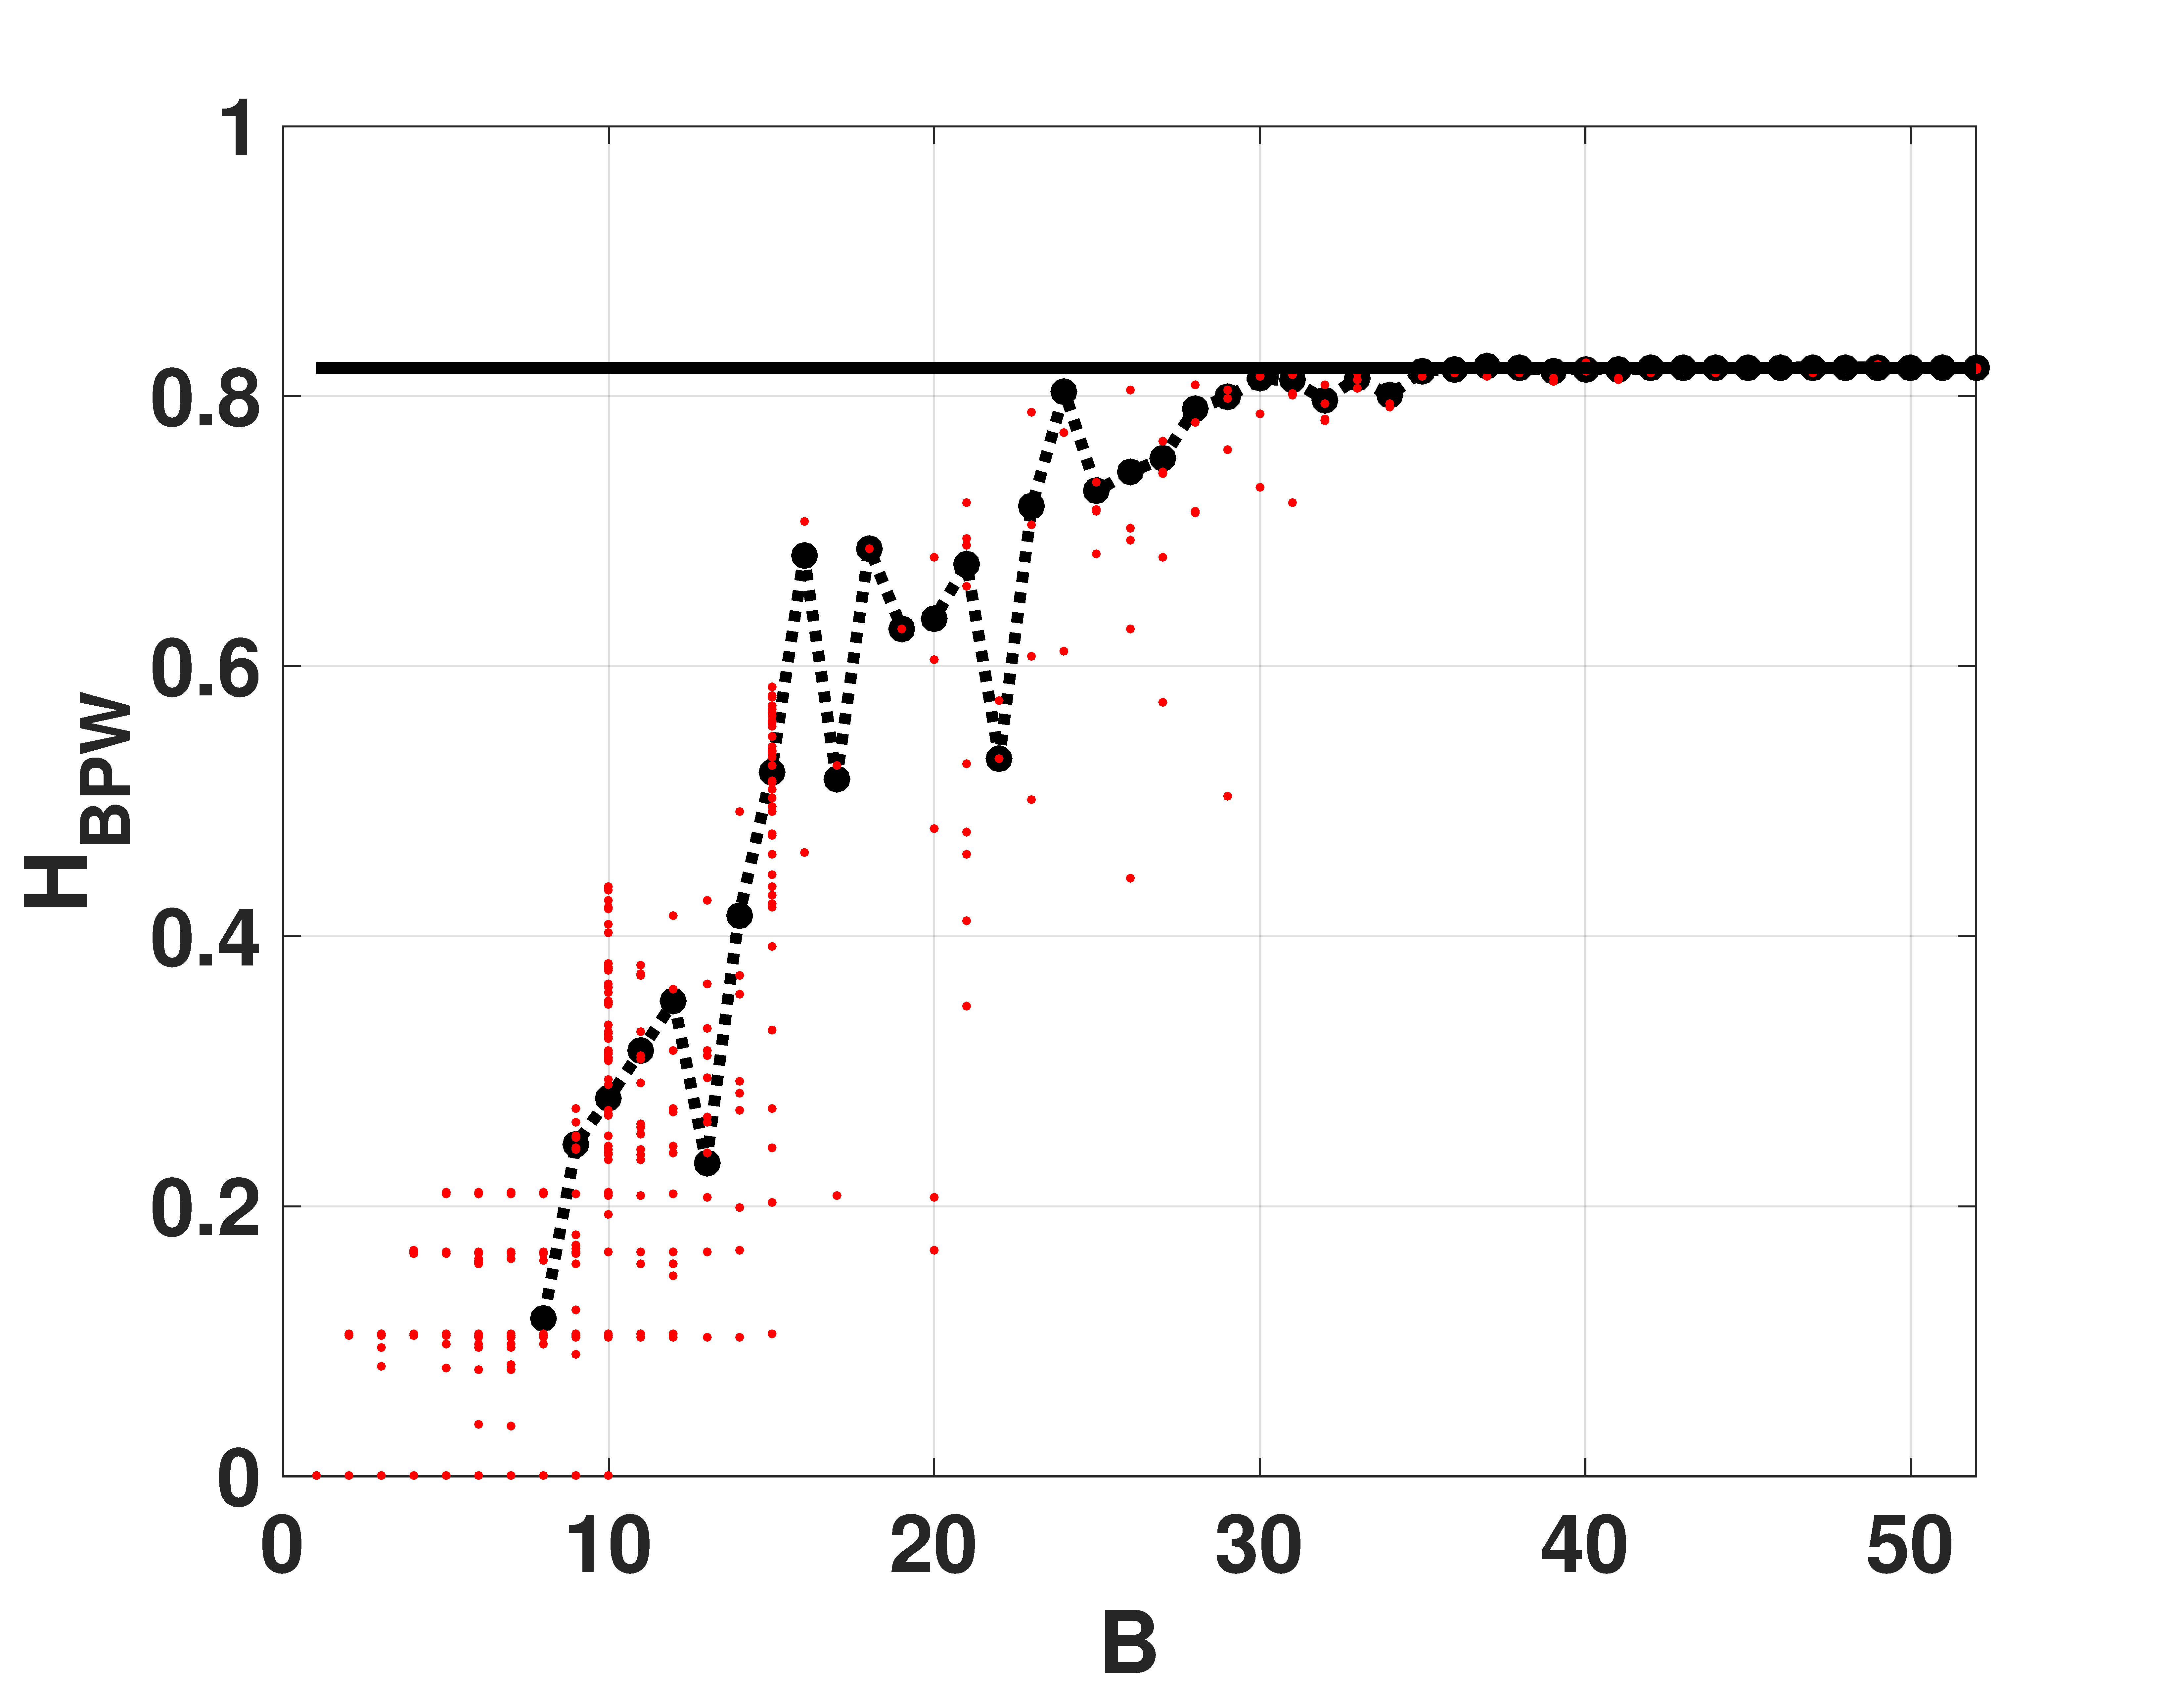
\includegraphics[width=\textwidth]{Hbpw_Even}
		\caption{$H_{BPW}$ vs. $B$}
		\label{fig:Hbpw_Even}
	\end{subfigure}
	\begin{subfigure}[b]{0.49\textwidth}
		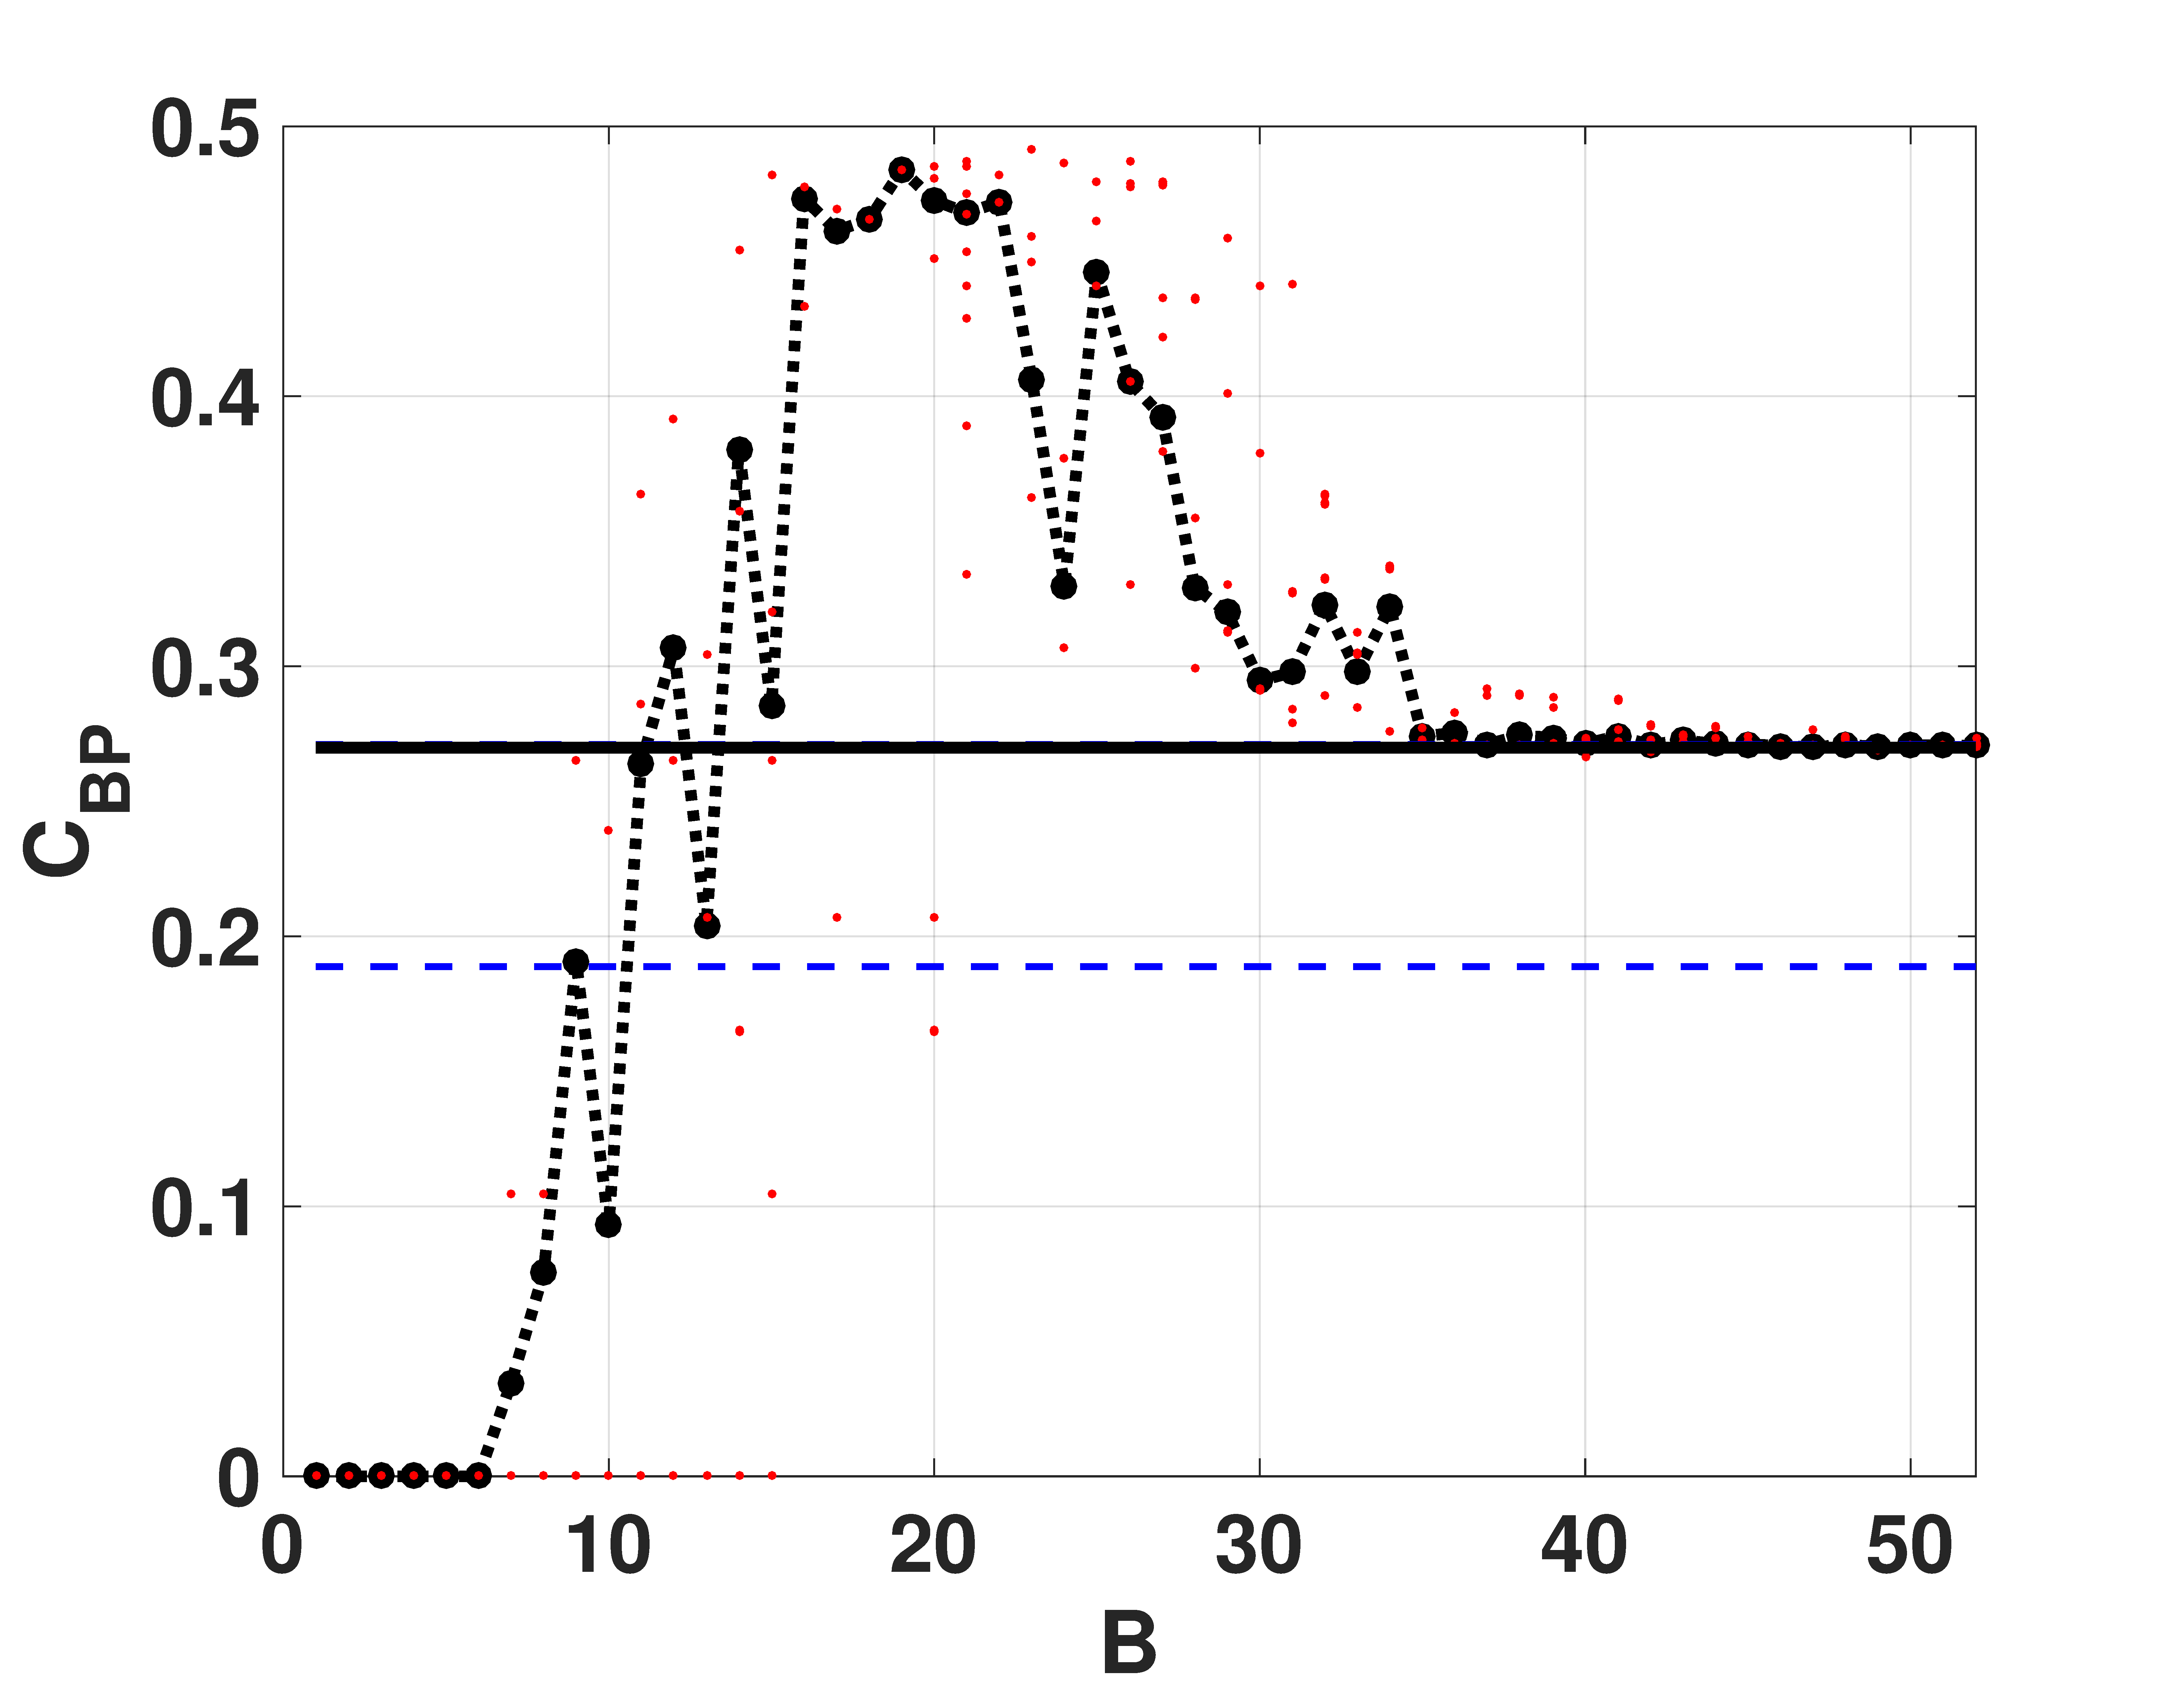
\includegraphics[width=\textwidth]{Cbp_Even}
		\caption{$C_{BP}$ vs. $B$}
		\label{fig:Cbp_Even}
	\end{subfigure}
	\begin{subfigure}[b]{0.49\textwidth}
		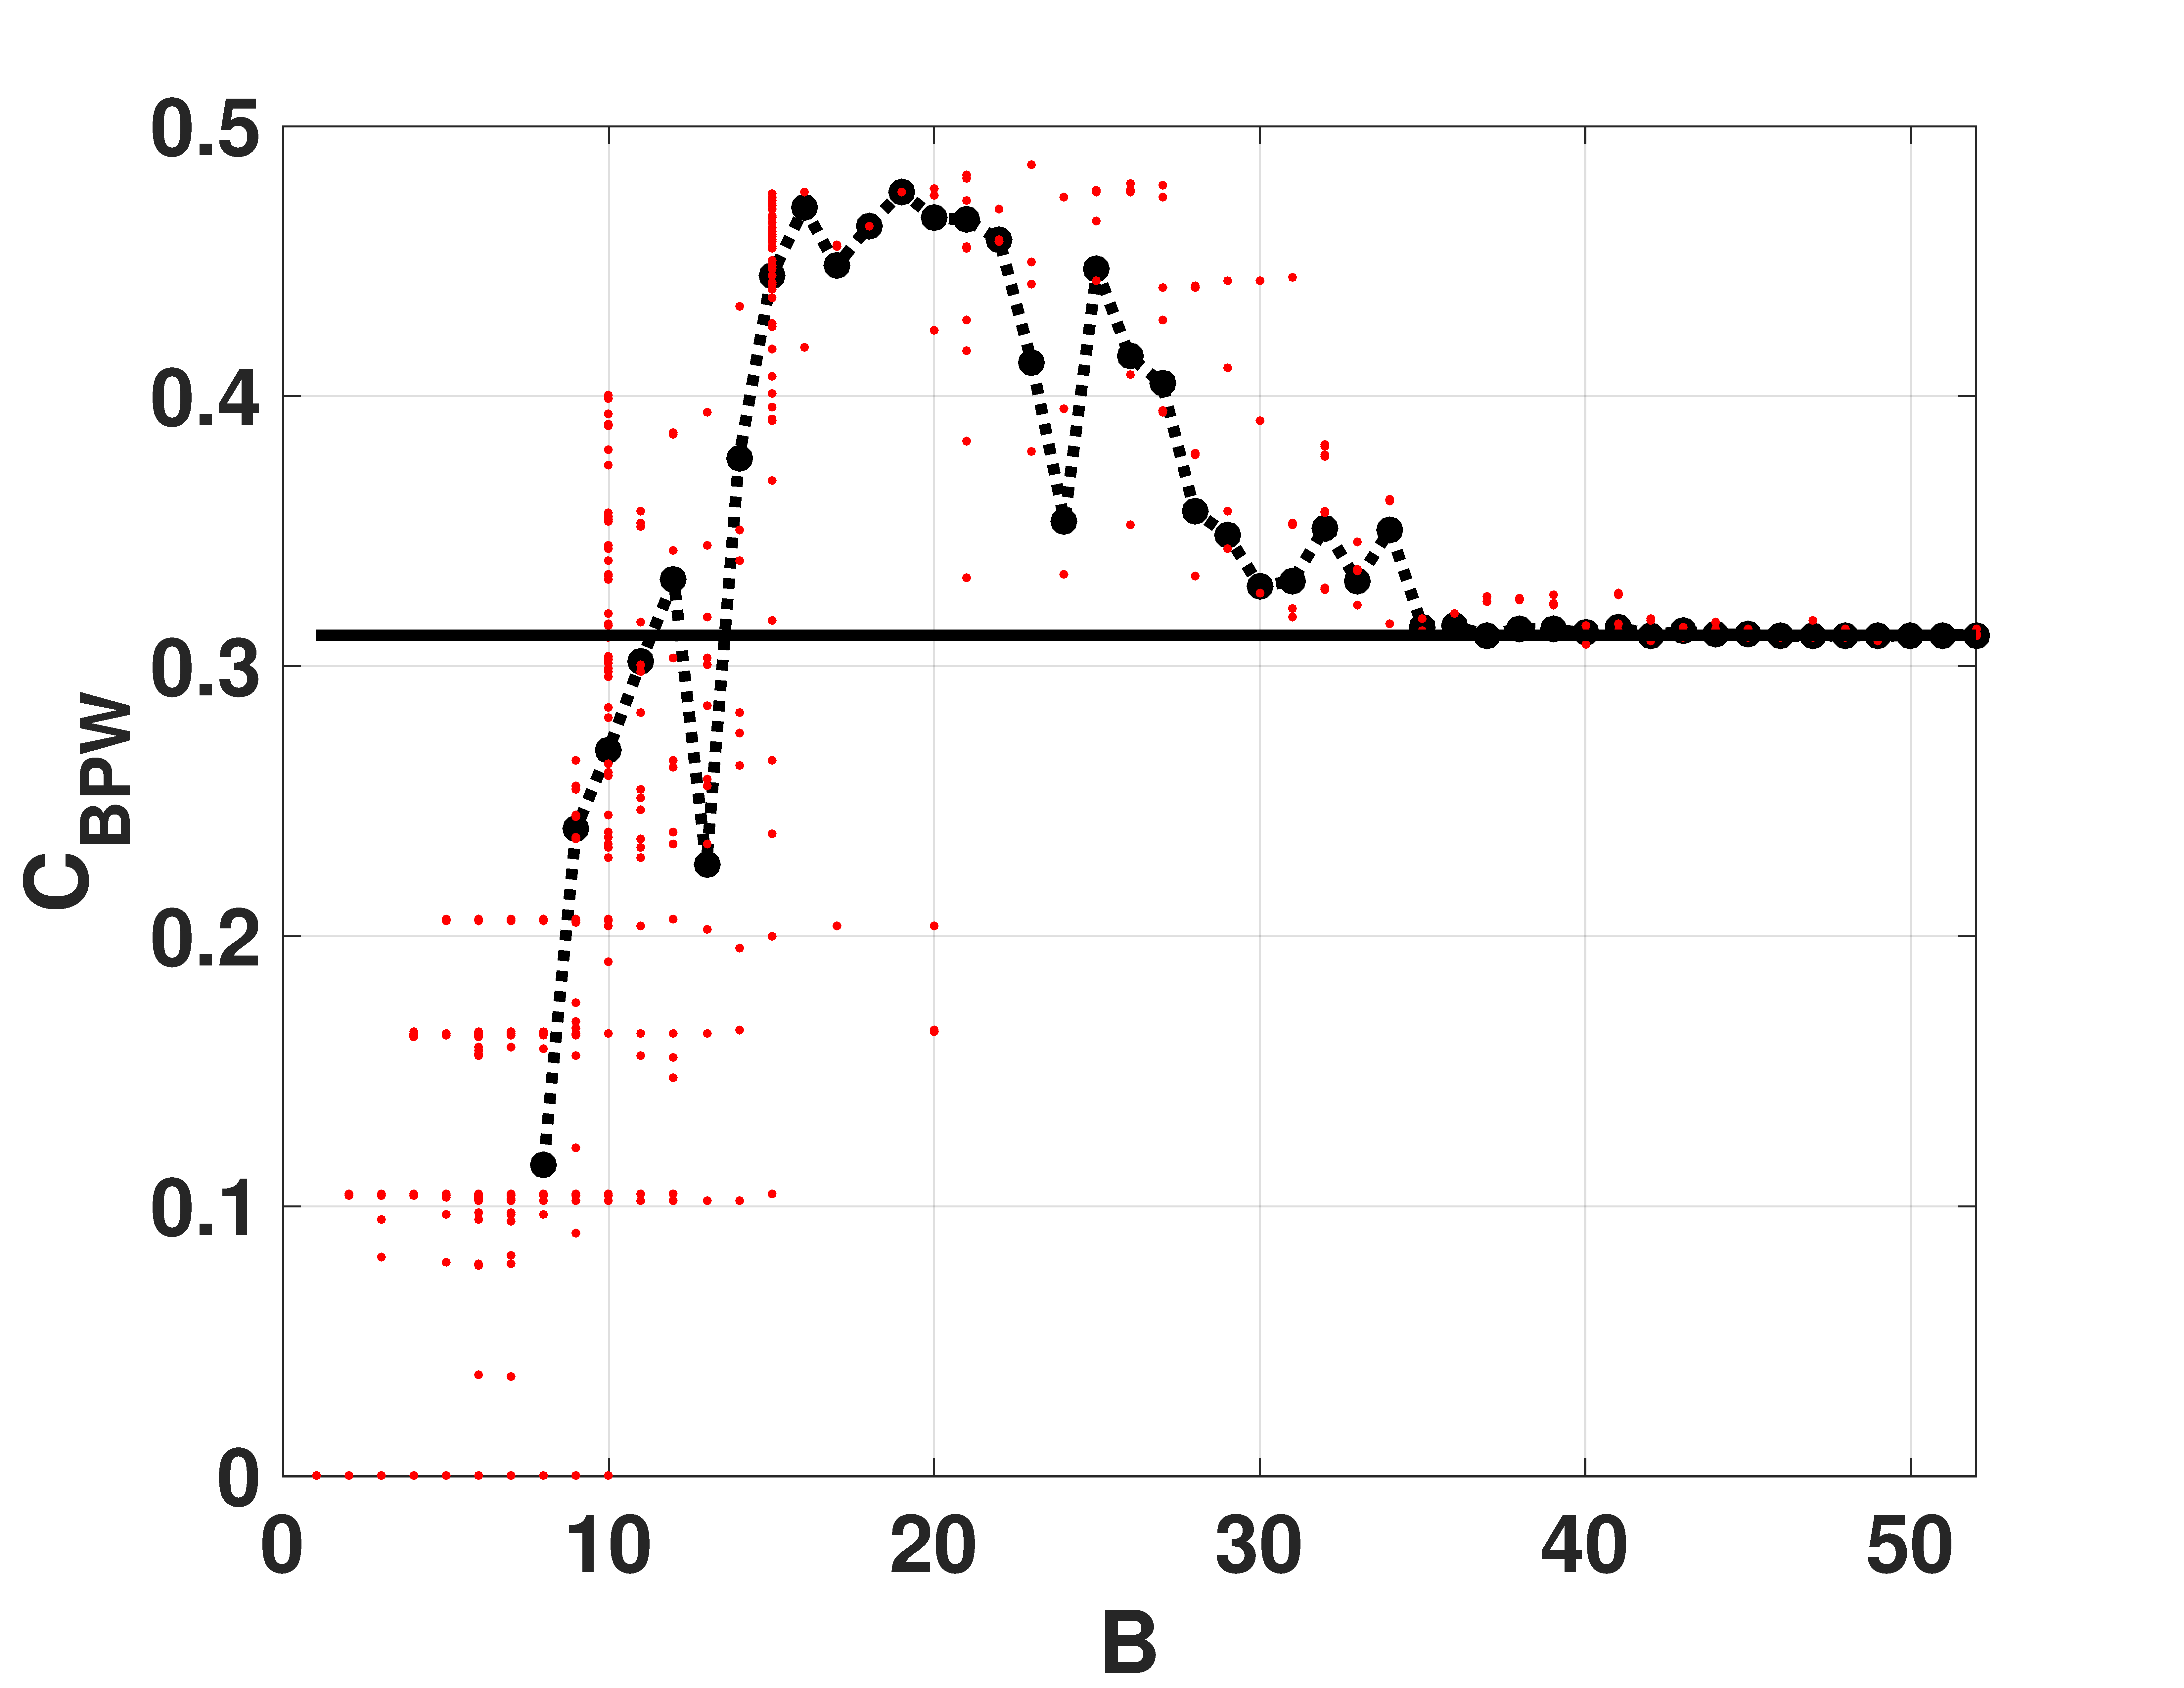
\includegraphics[width=\textwidth]{Cbpw_Even}
		\caption{$C_{BPW}$ vs. $B$}
		\label{fig:Cbpw_Even}
	\end{subfigure}
	\begin{subfigure}[b]{0.49\textwidth}
		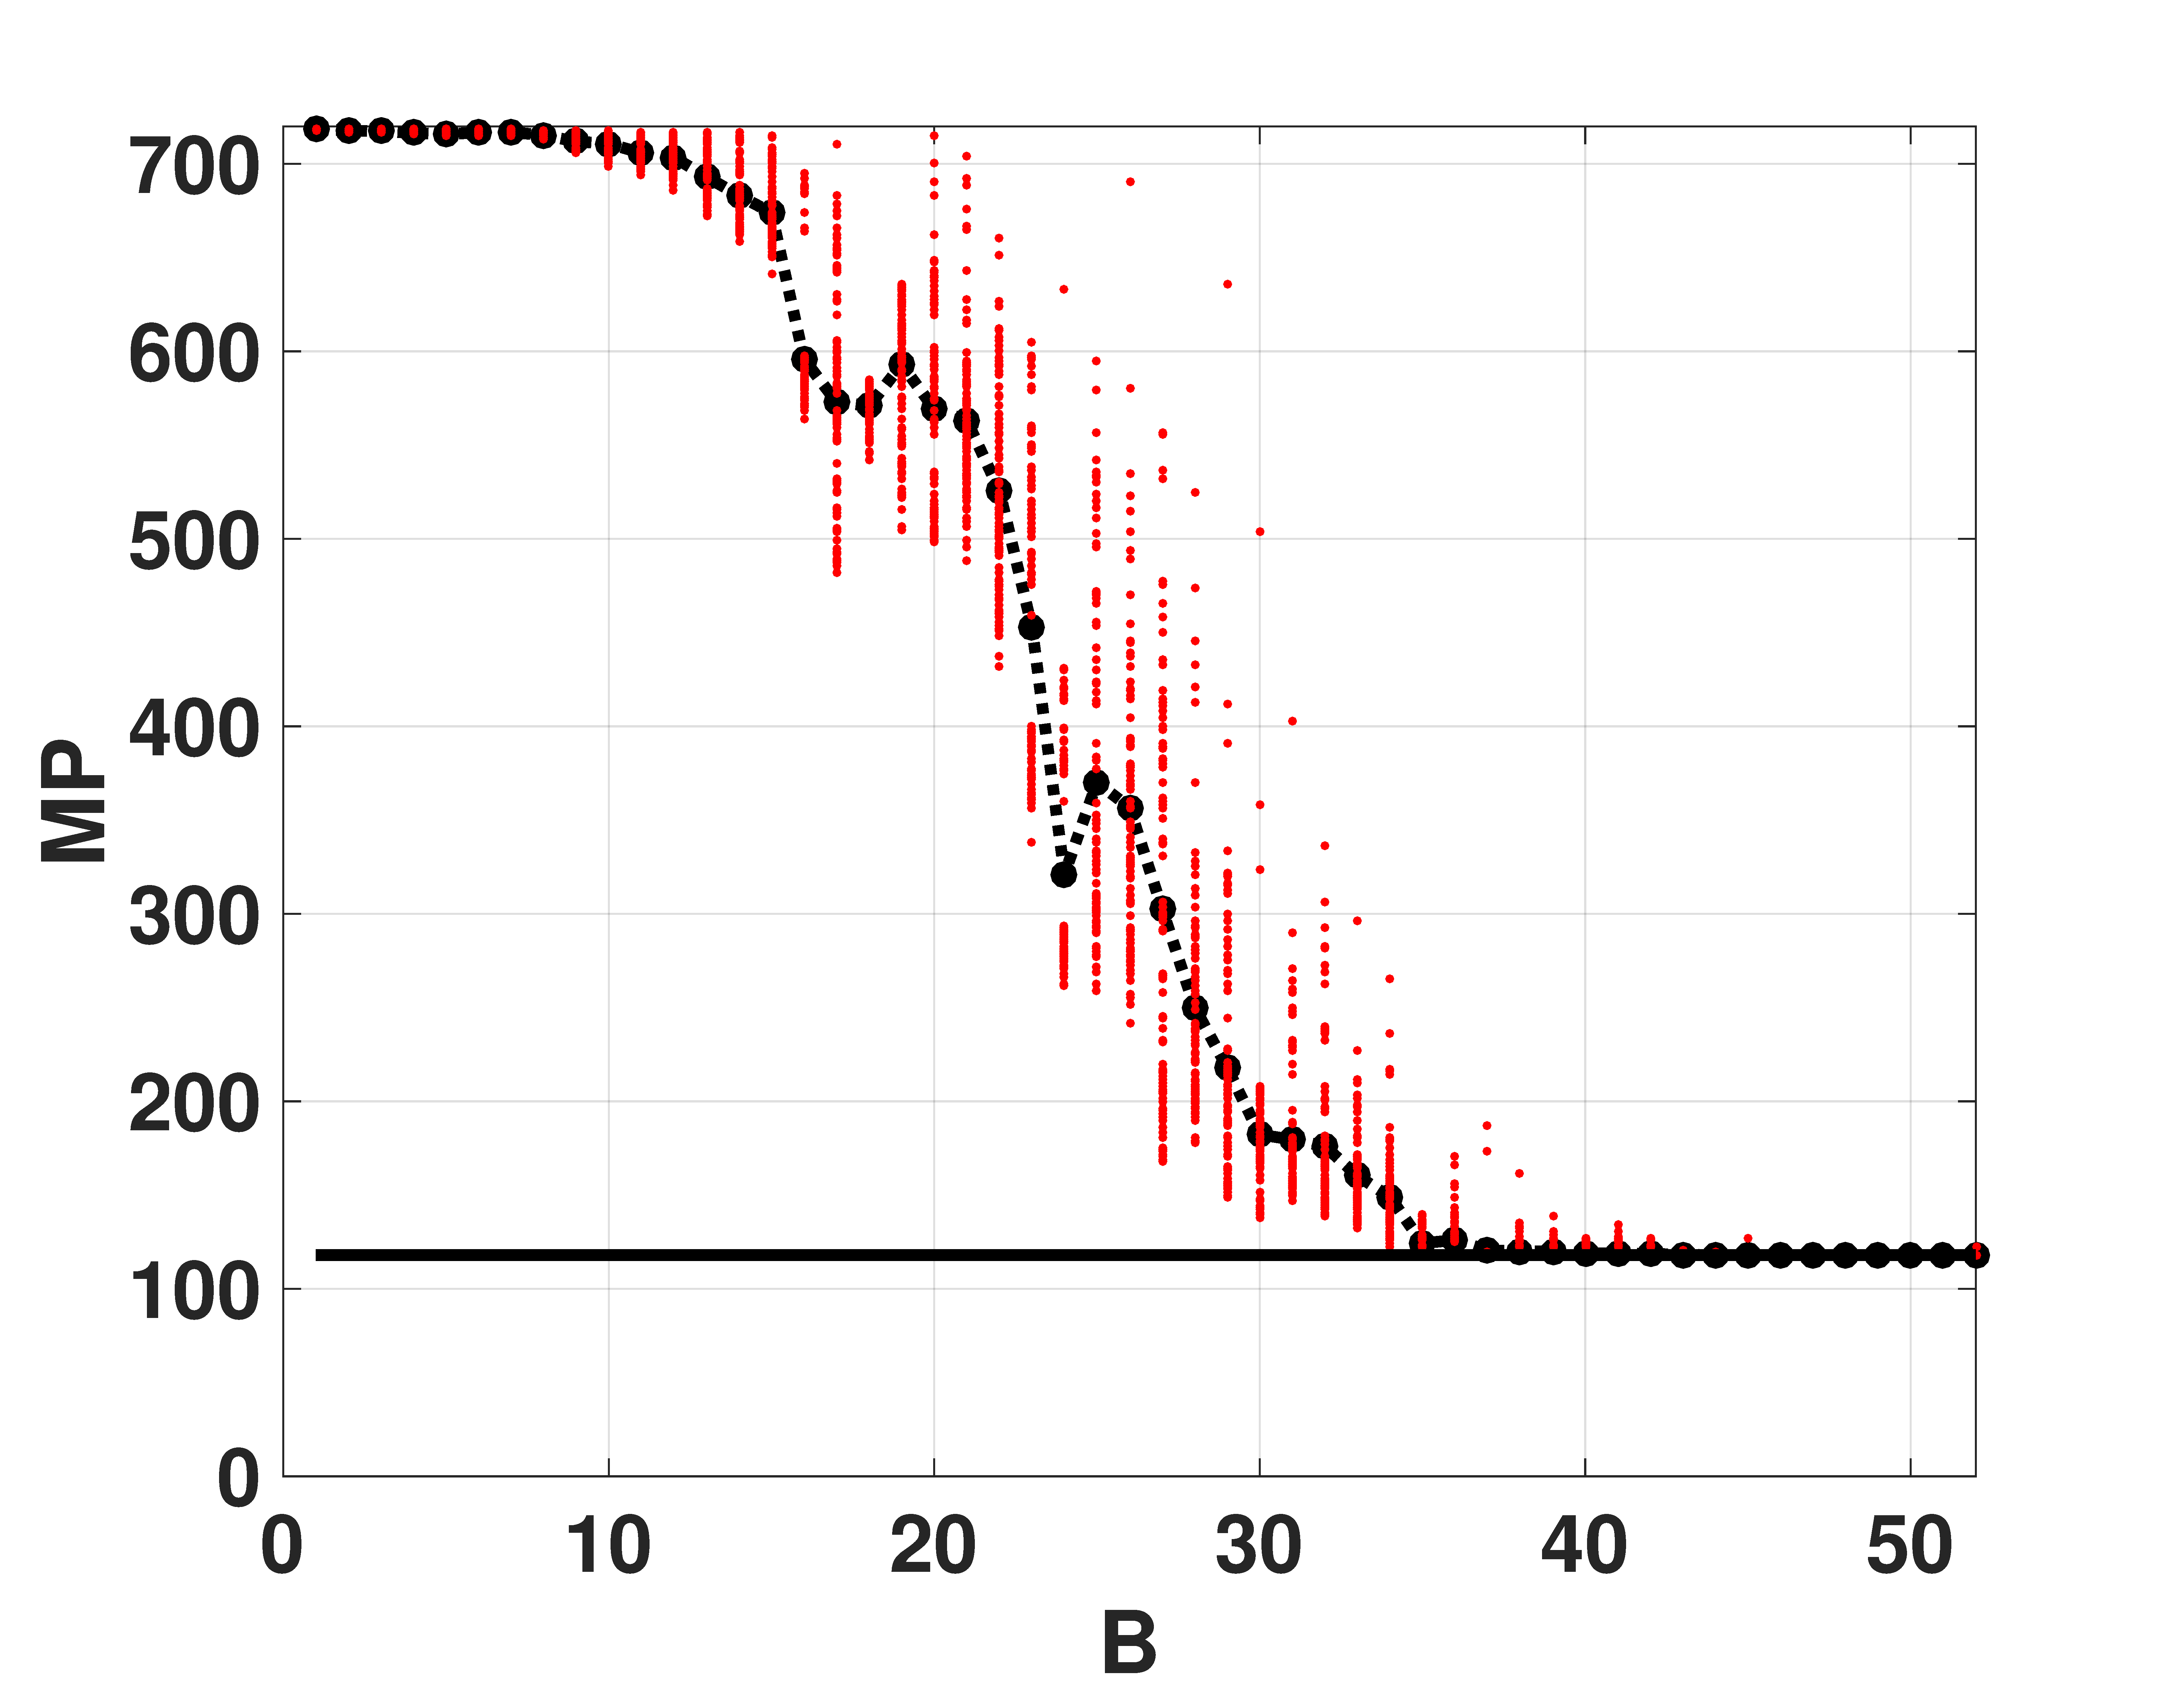
\includegraphics[width=\textwidth]{MP_Even}
		\caption{MP vs. $B$}
		\label{fig:MP_Even}
	\end{subfigure}
	\caption{Propiedades estadísticas para el mapa EVEN}
	\label{fig:EVEN_QuantiB}
\end{figure}
%
\begin{figure}[htpb]
	\centering
	\begin{subfigure}[b]{0.49\textwidth}
		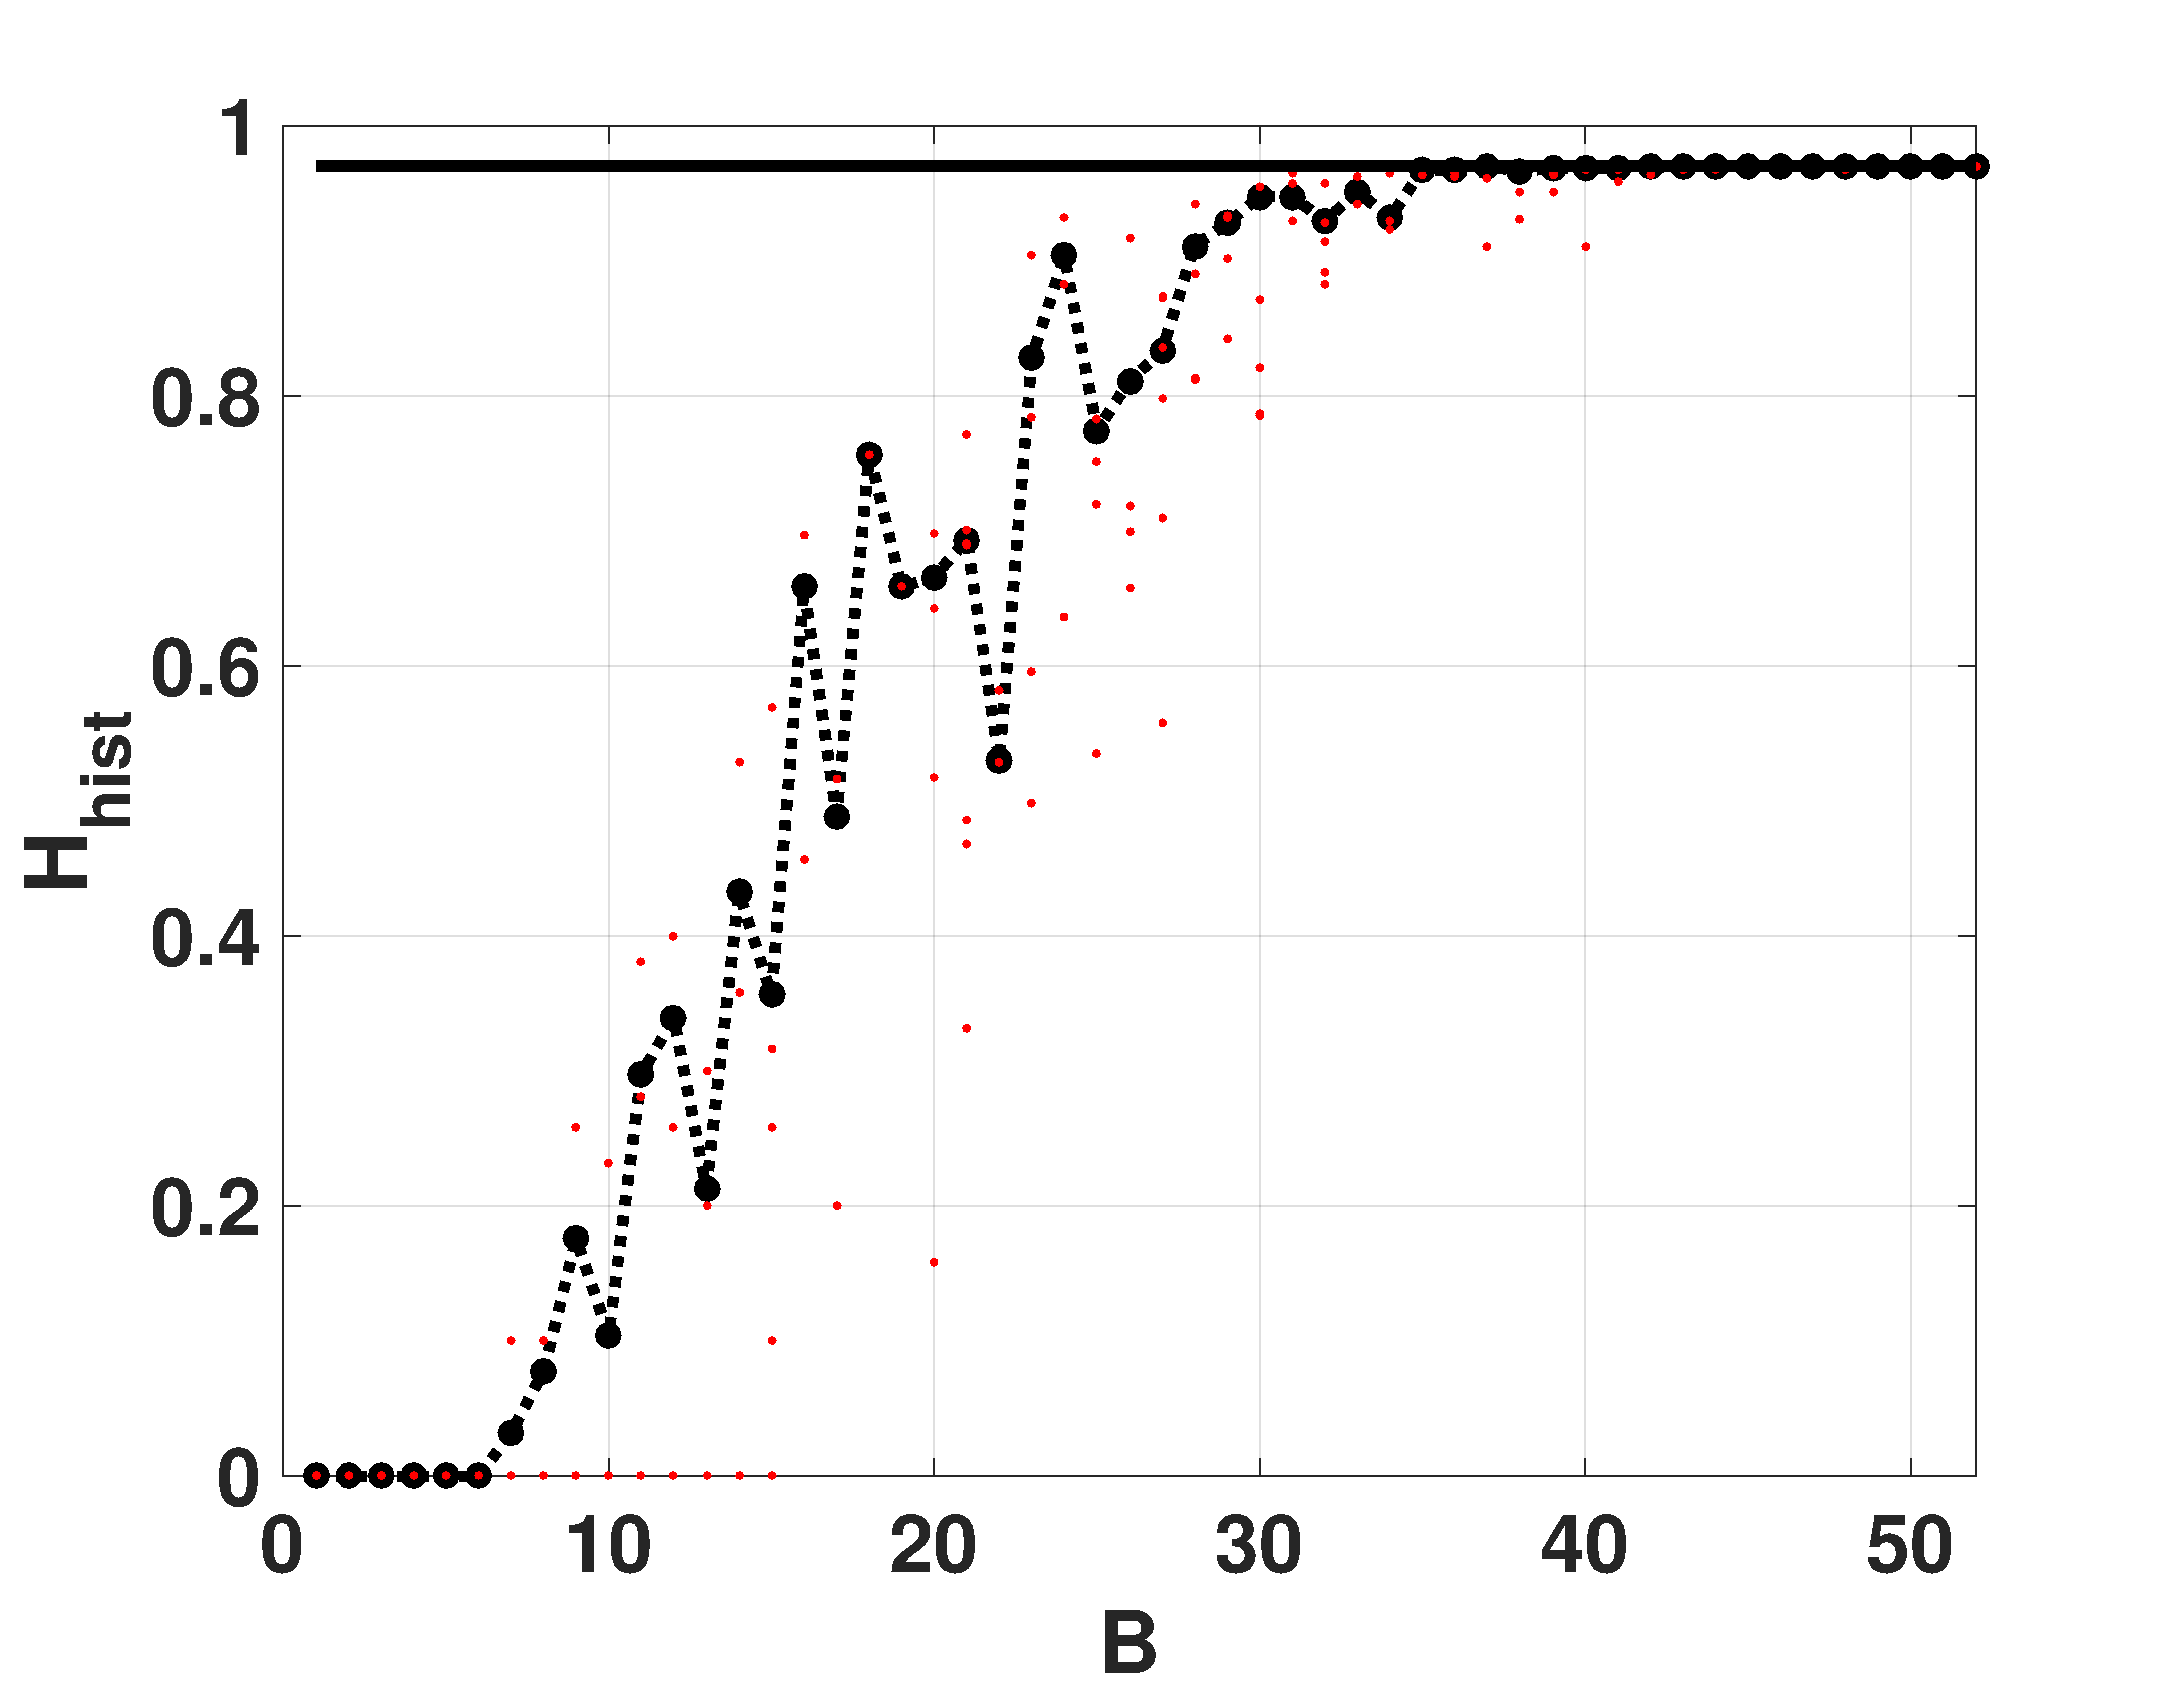
\includegraphics[width=\textwidth]{Hval_Odd}
		\caption{$H_{hist}$ vs. $B$}
		\label{fig:Hval_Odd}
	\end{subfigure}
	\begin{subfigure}[b]{0.49\textwidth}
		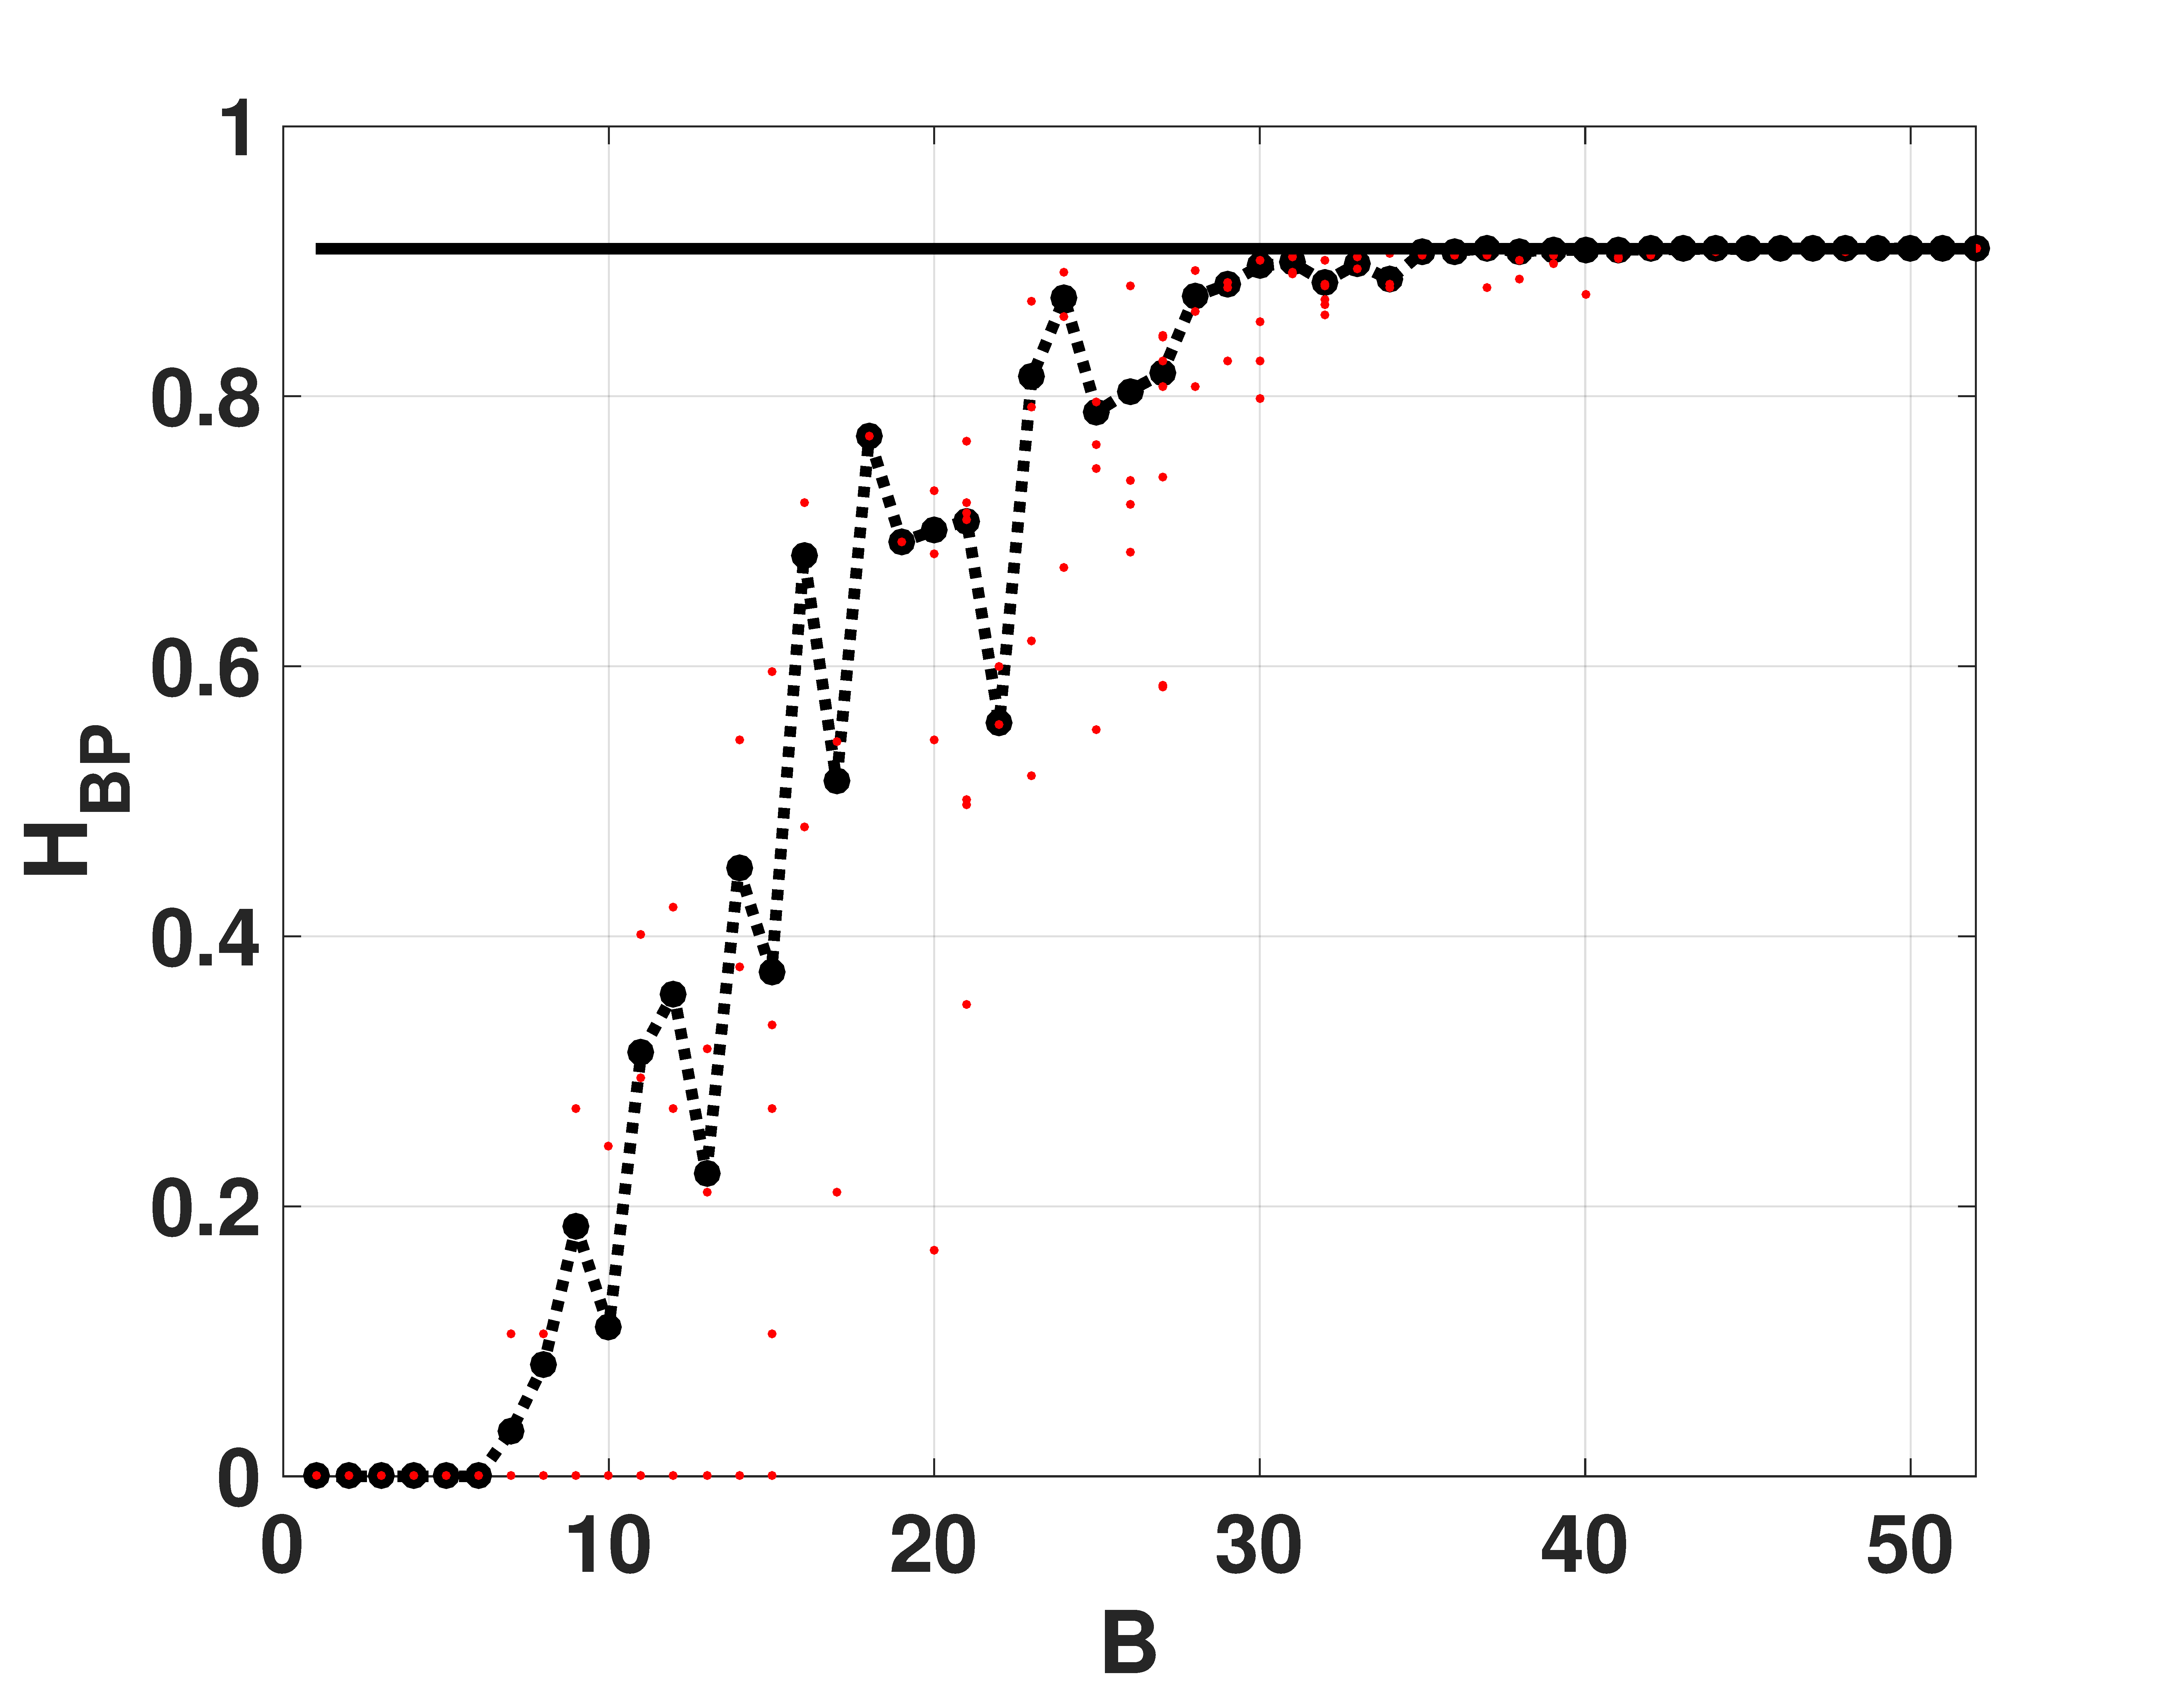
\includegraphics[width=\textwidth]{Hbp_Odd}
		\caption{$H_{BP}$ vs. $B$}
		\label{fig:Hbp_Odd}
	\end{subfigure}
	\begin{subfigure}[b]{0.49\textwidth}
		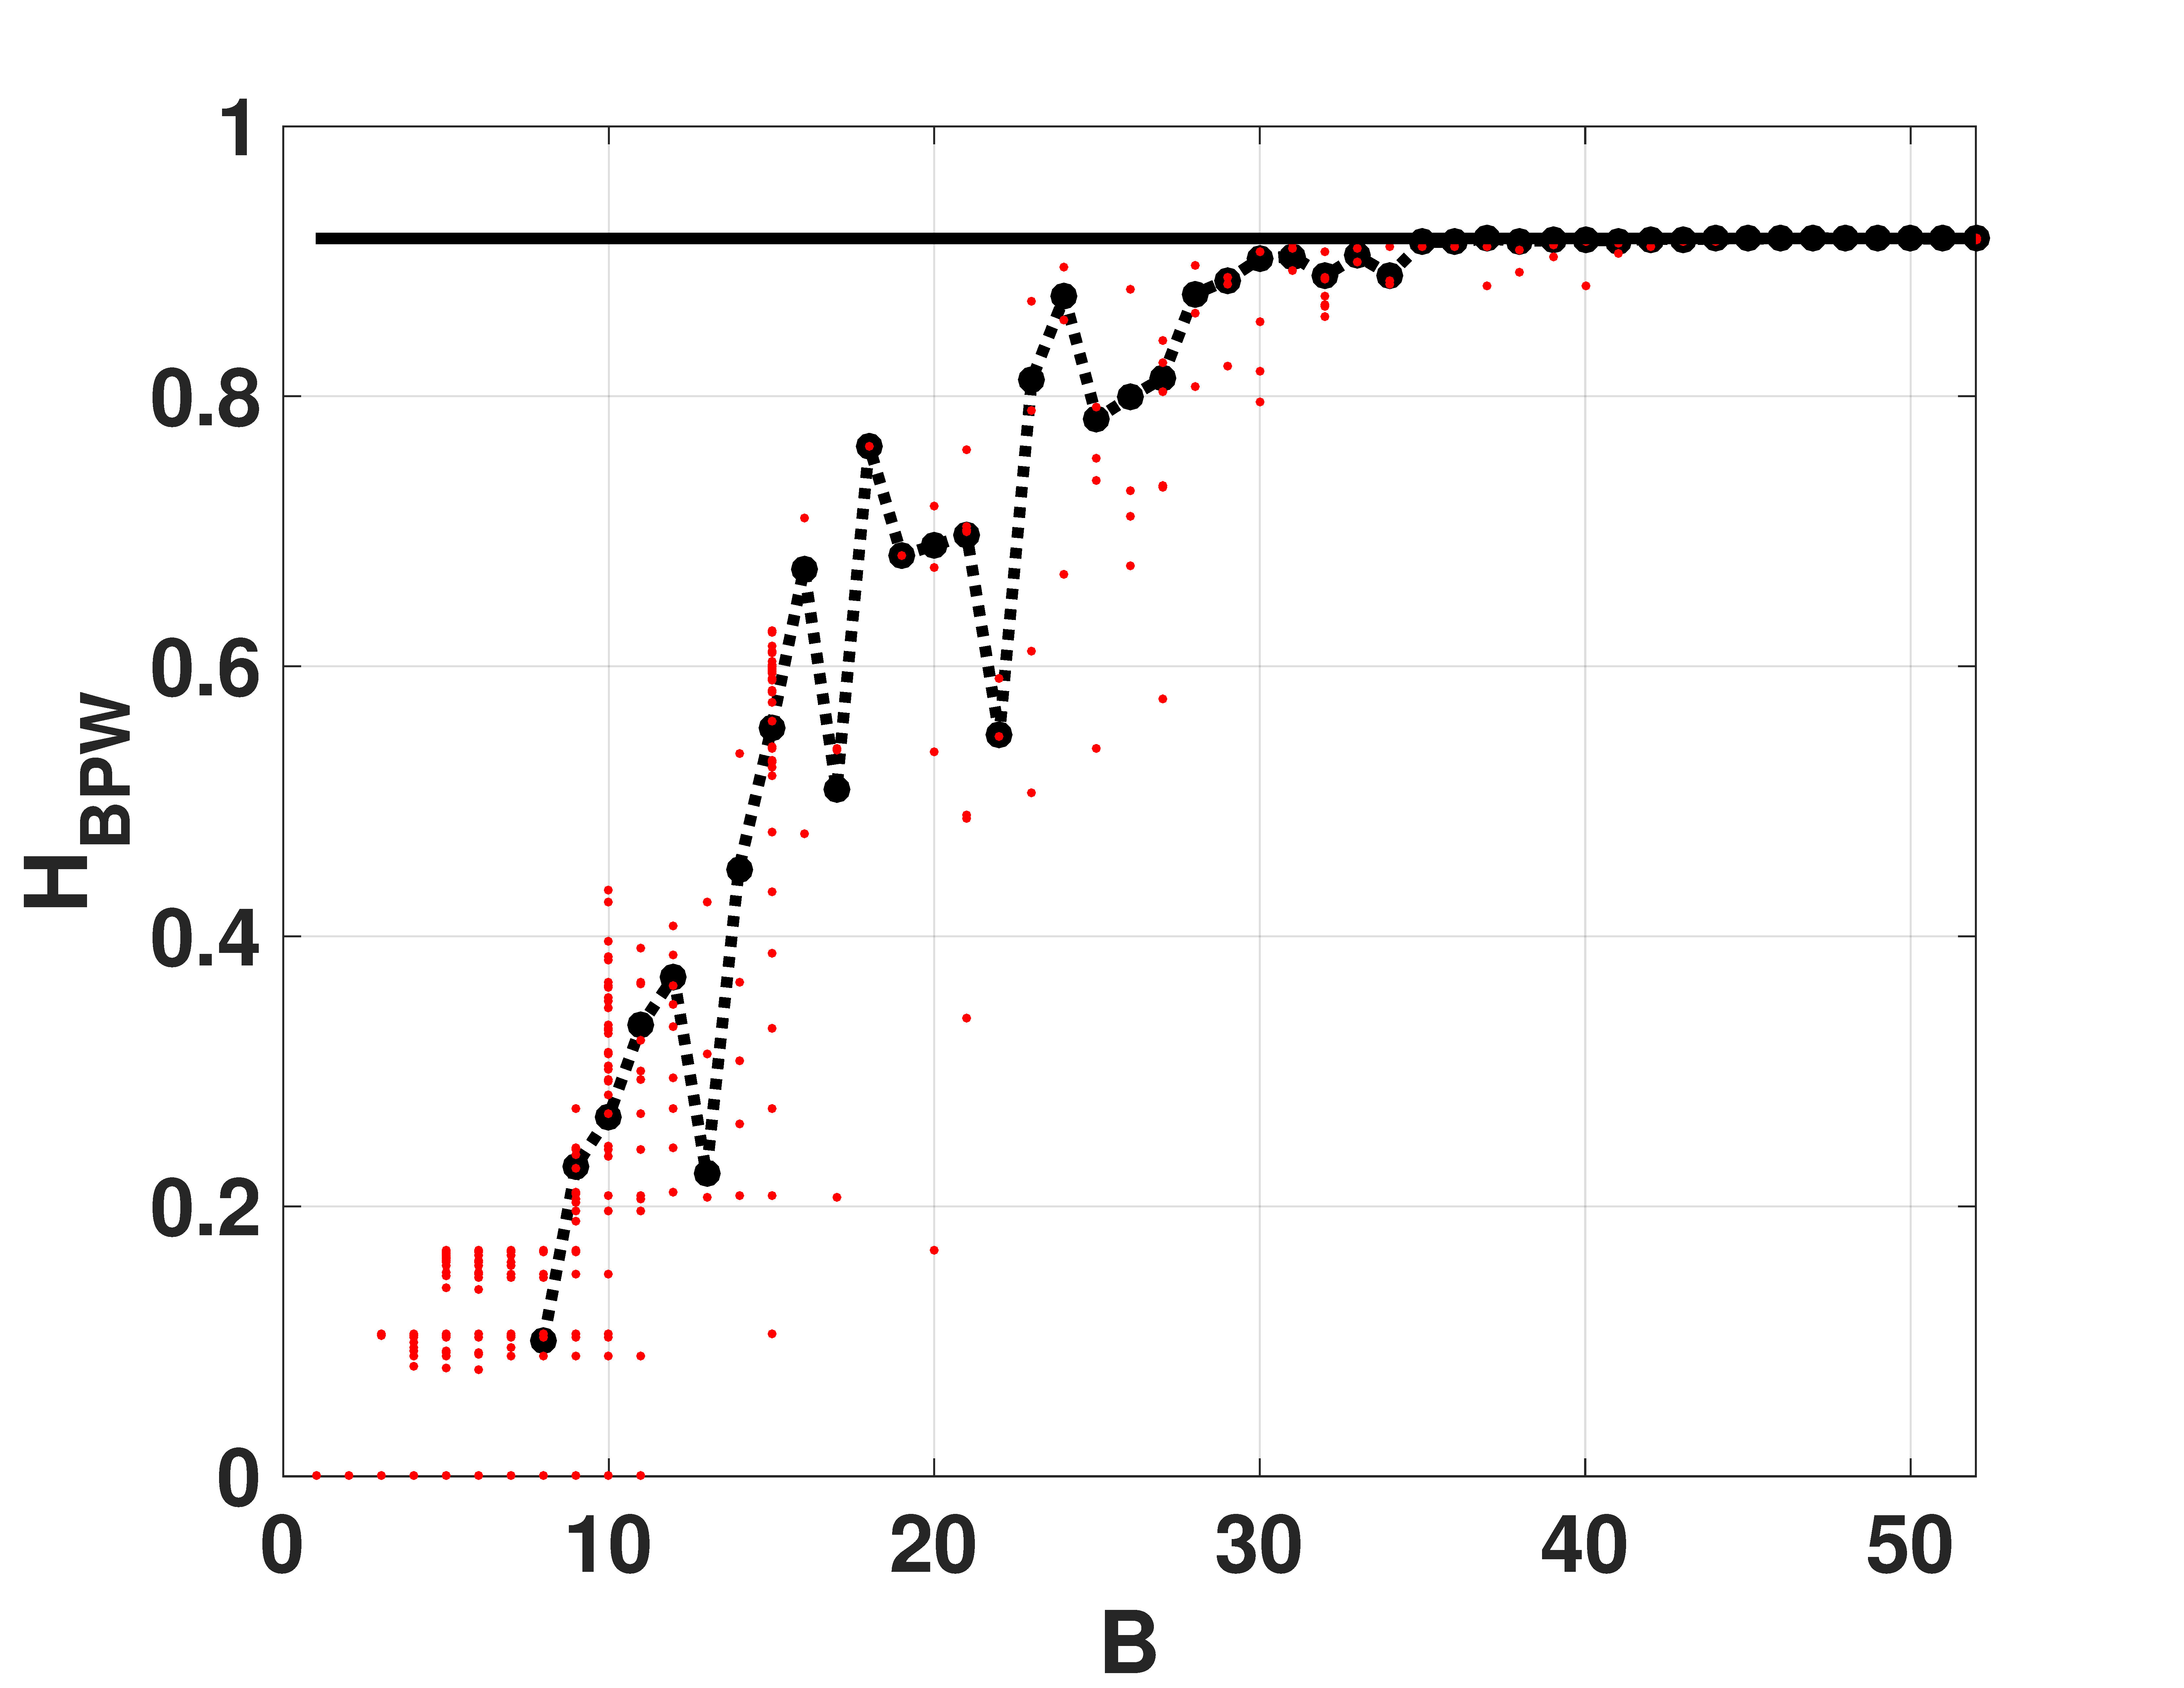
\includegraphics[width=\textwidth]{Hbpw_Odd}
		\caption{$H_{BPW}$ vs. $B$}
		\label{fig:Hbpw_Odd}
	\end{subfigure}
	\begin{subfigure}[b]{0.49\textwidth}
		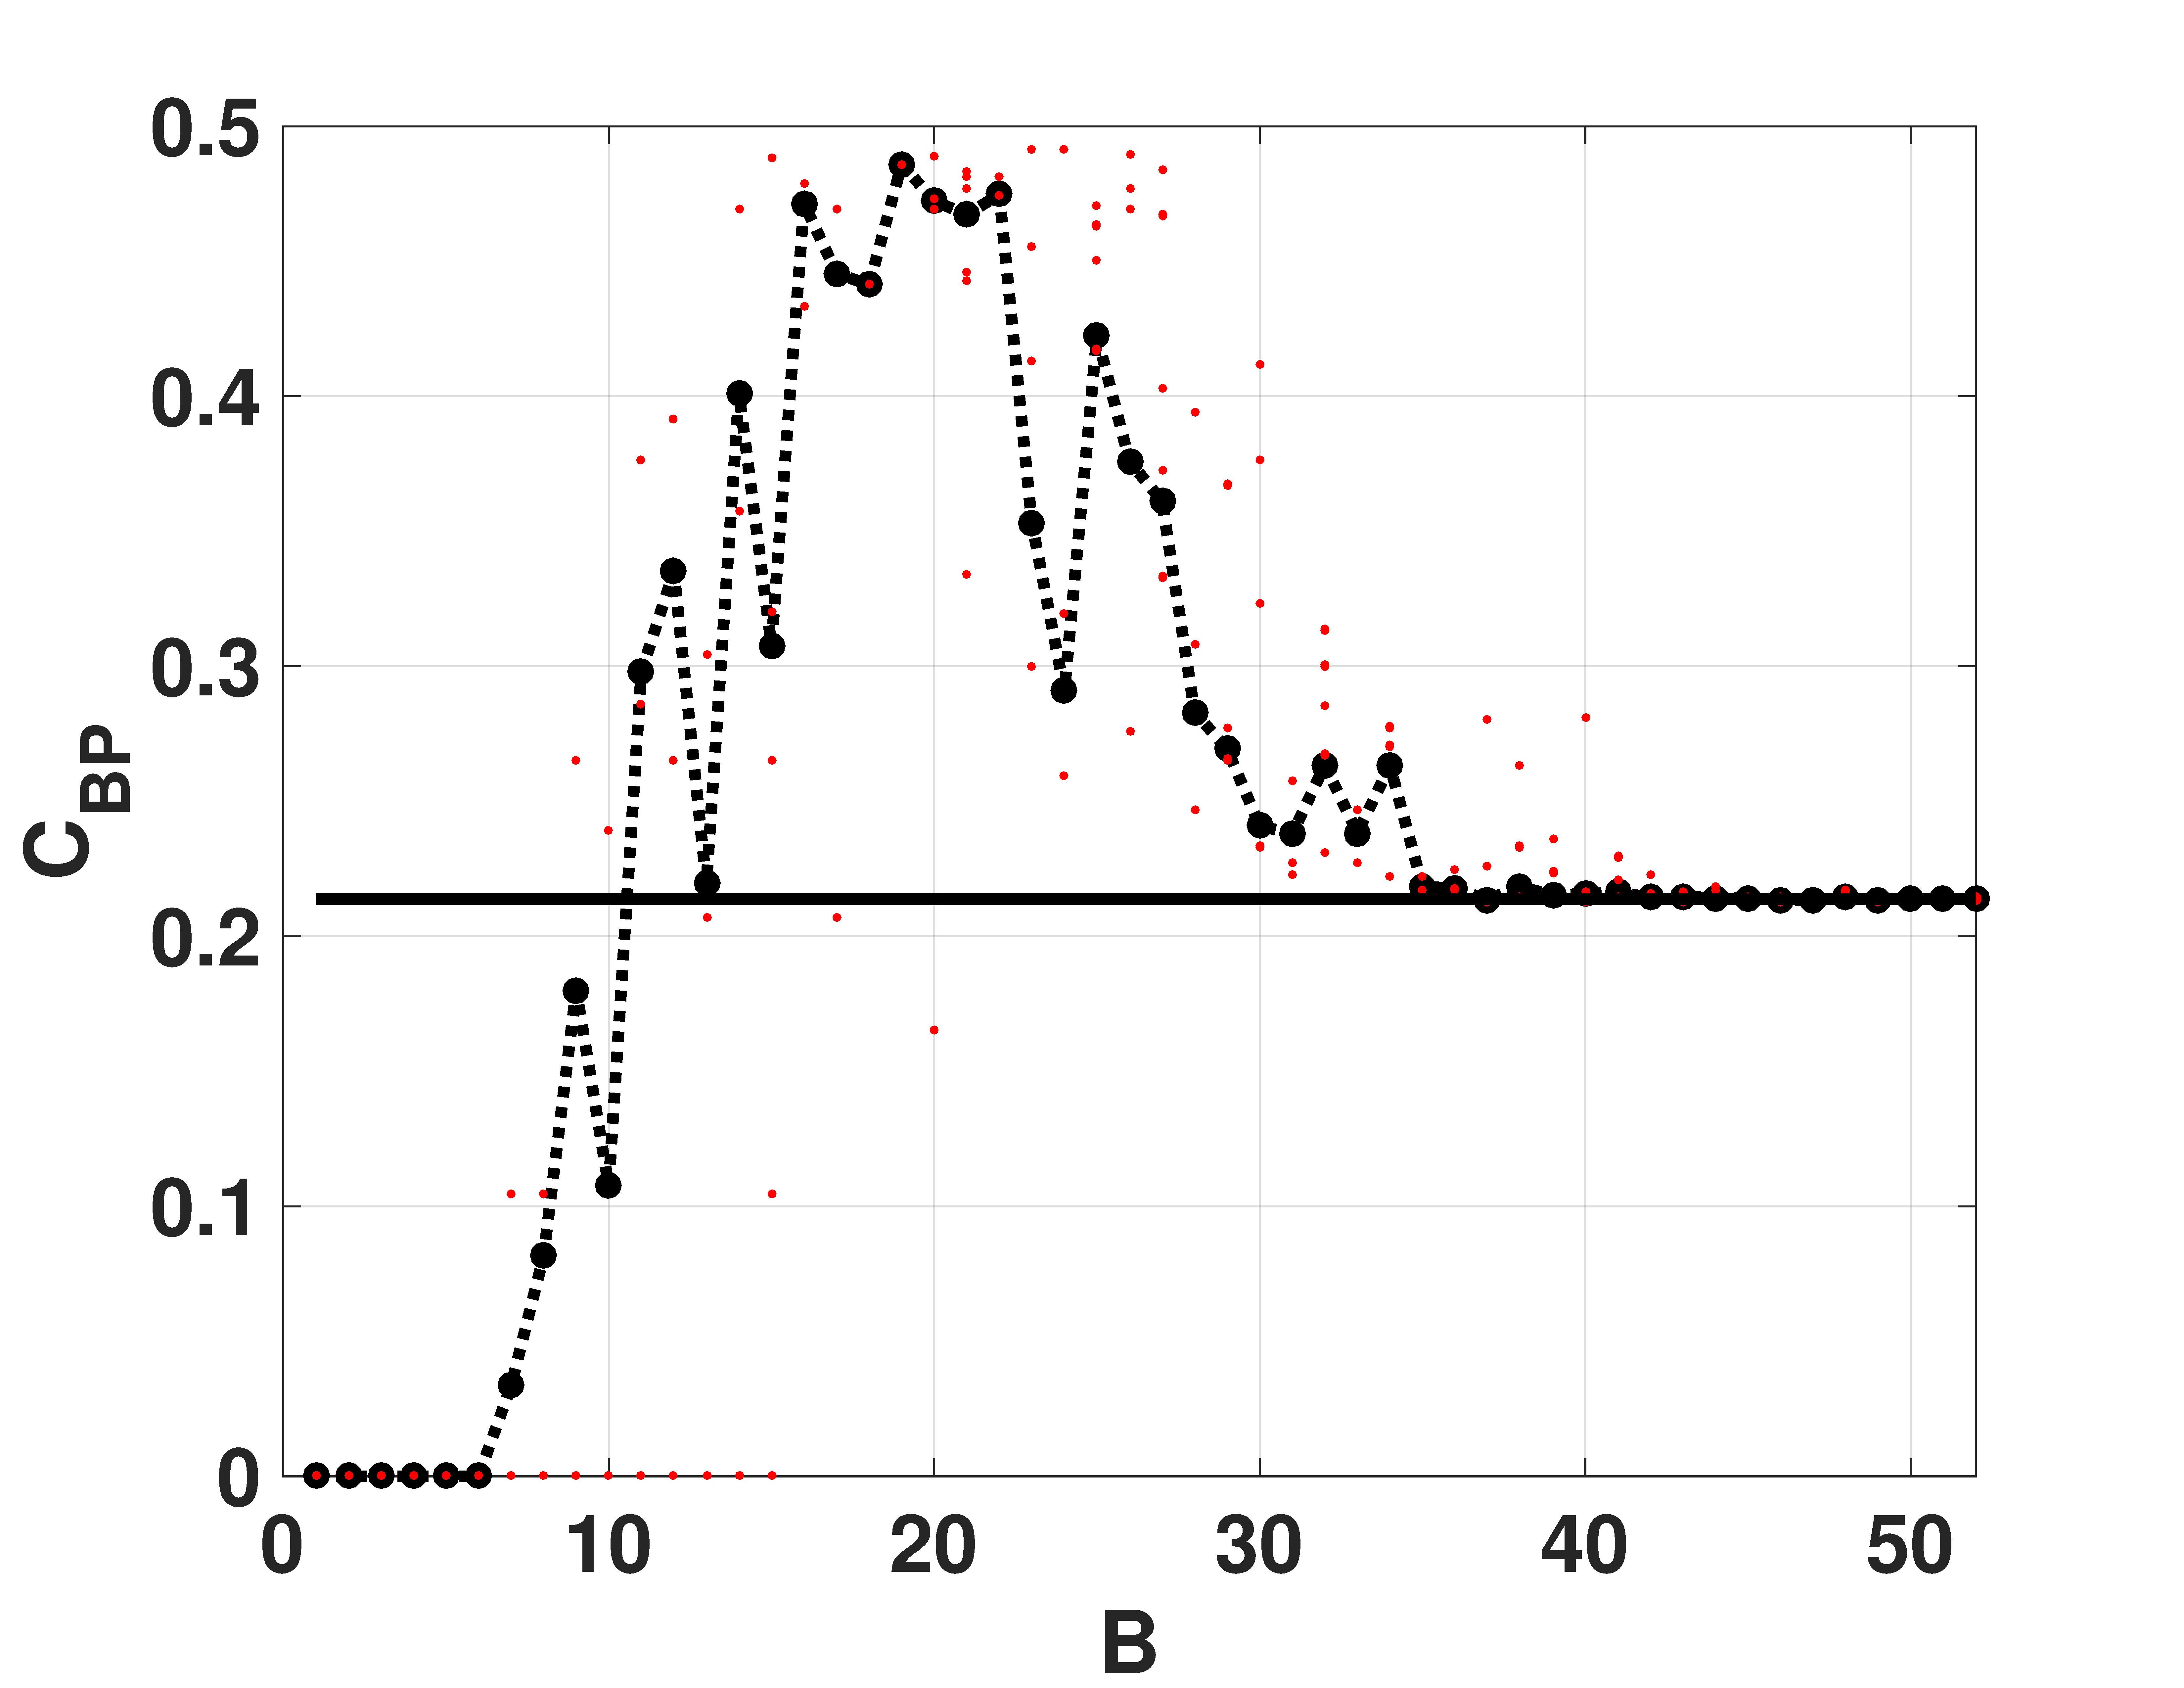
\includegraphics[width=\textwidth]{Cbp_Odd}
		\caption{$C_{BP}$ vs. $B$}
		\label{fig:Cbp_Odd}
	\end{subfigure}
	\begin{subfigure}[b]{0.49\textwidth}
		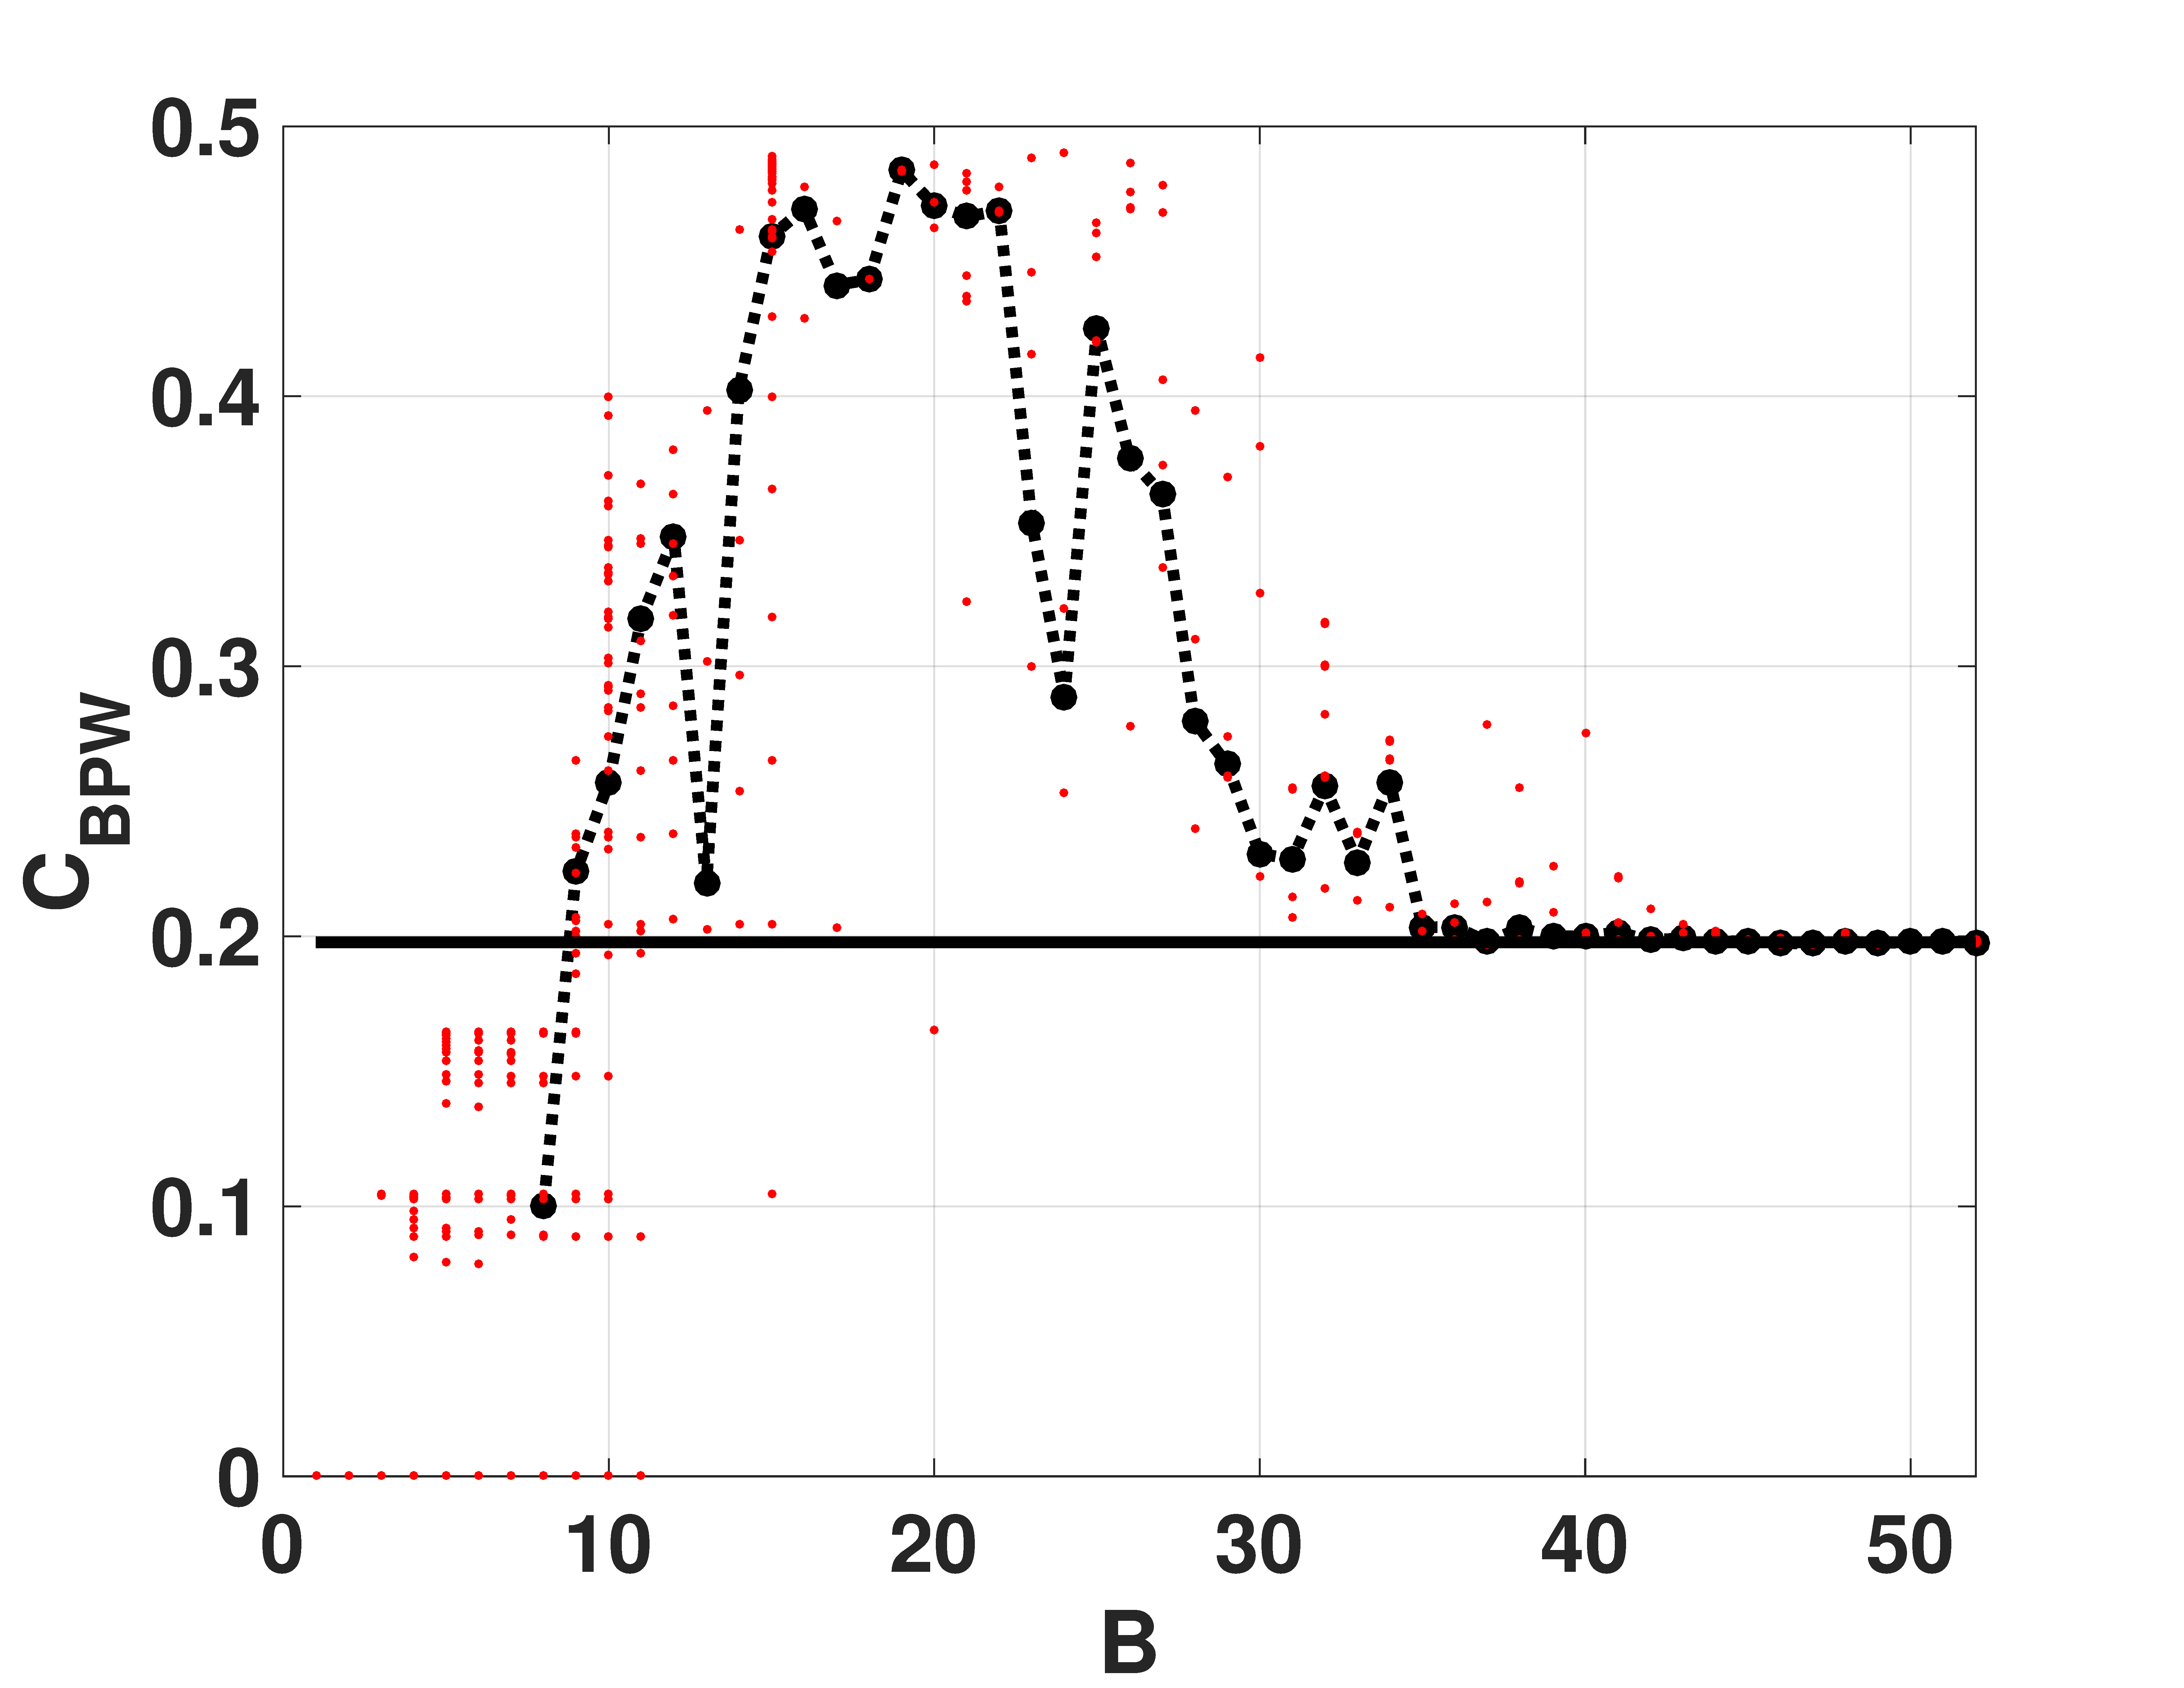
\includegraphics[width=\textwidth]{Cbpw_Odd}
		\caption{$C_{BPW}$ vs. $B$}
		\label{fig:Cbpw_Odd}
	\end{subfigure}
	\begin{subfigure}[b]{0.49\textwidth}
		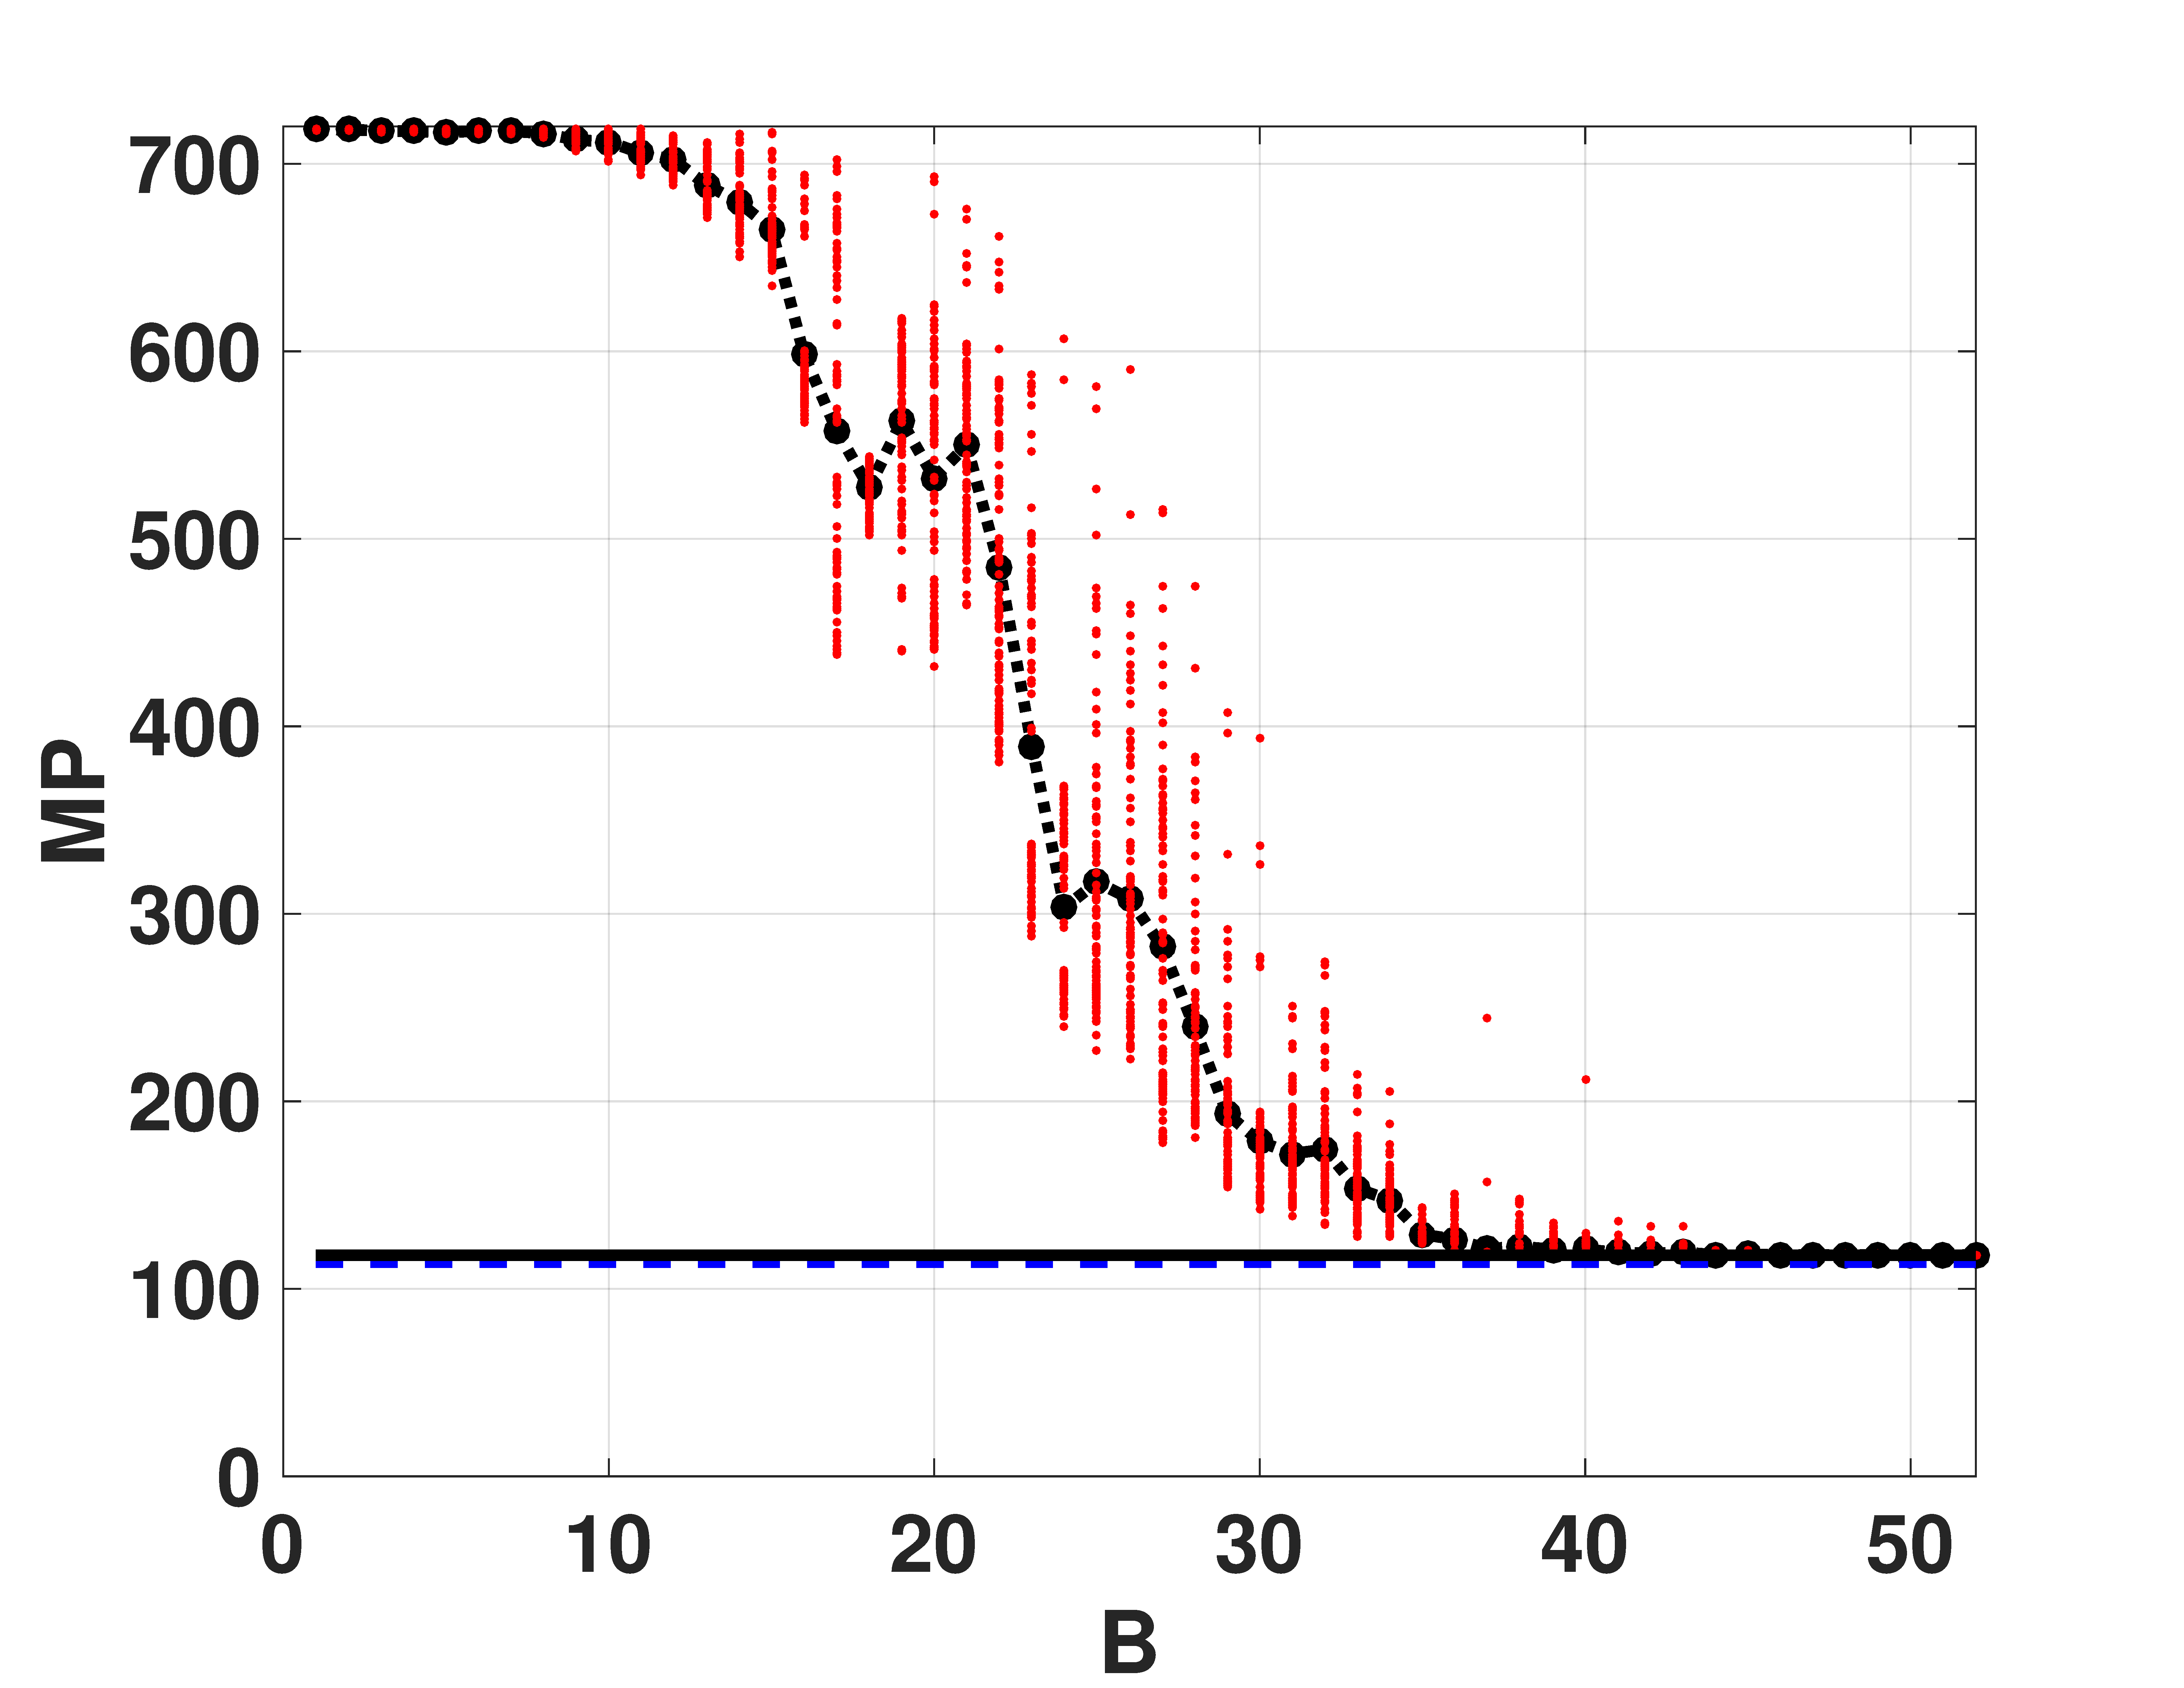
\includegraphics[width=\textwidth]{MP_Odd}
		\caption{MP vs. $B$}
		\label{fig:MP_Odd}
	\end{subfigure}
	\caption{Propiedades estadísticas para el mapa ODD}
	\label{fig:ODD_QuantiB}
\end{figure}

La mejora mostrada en las figuras \ref{fig:EVEN_QuantiB} y \ref{fig:ODD_QuantiB} se refleja en la posición del punto asintótico en los planos \ref{fig: EVEN_HH}, y \ref{fig:ODD_HH}.
En ambos casos, esta posición es la más cercana al punto ideal $(H_{hist}, H_{BP}) = (1, 1)$, porque los vectores resultantes presentan una mejor mezcla.
%
\begin{figure}[htpb]
	\centering
	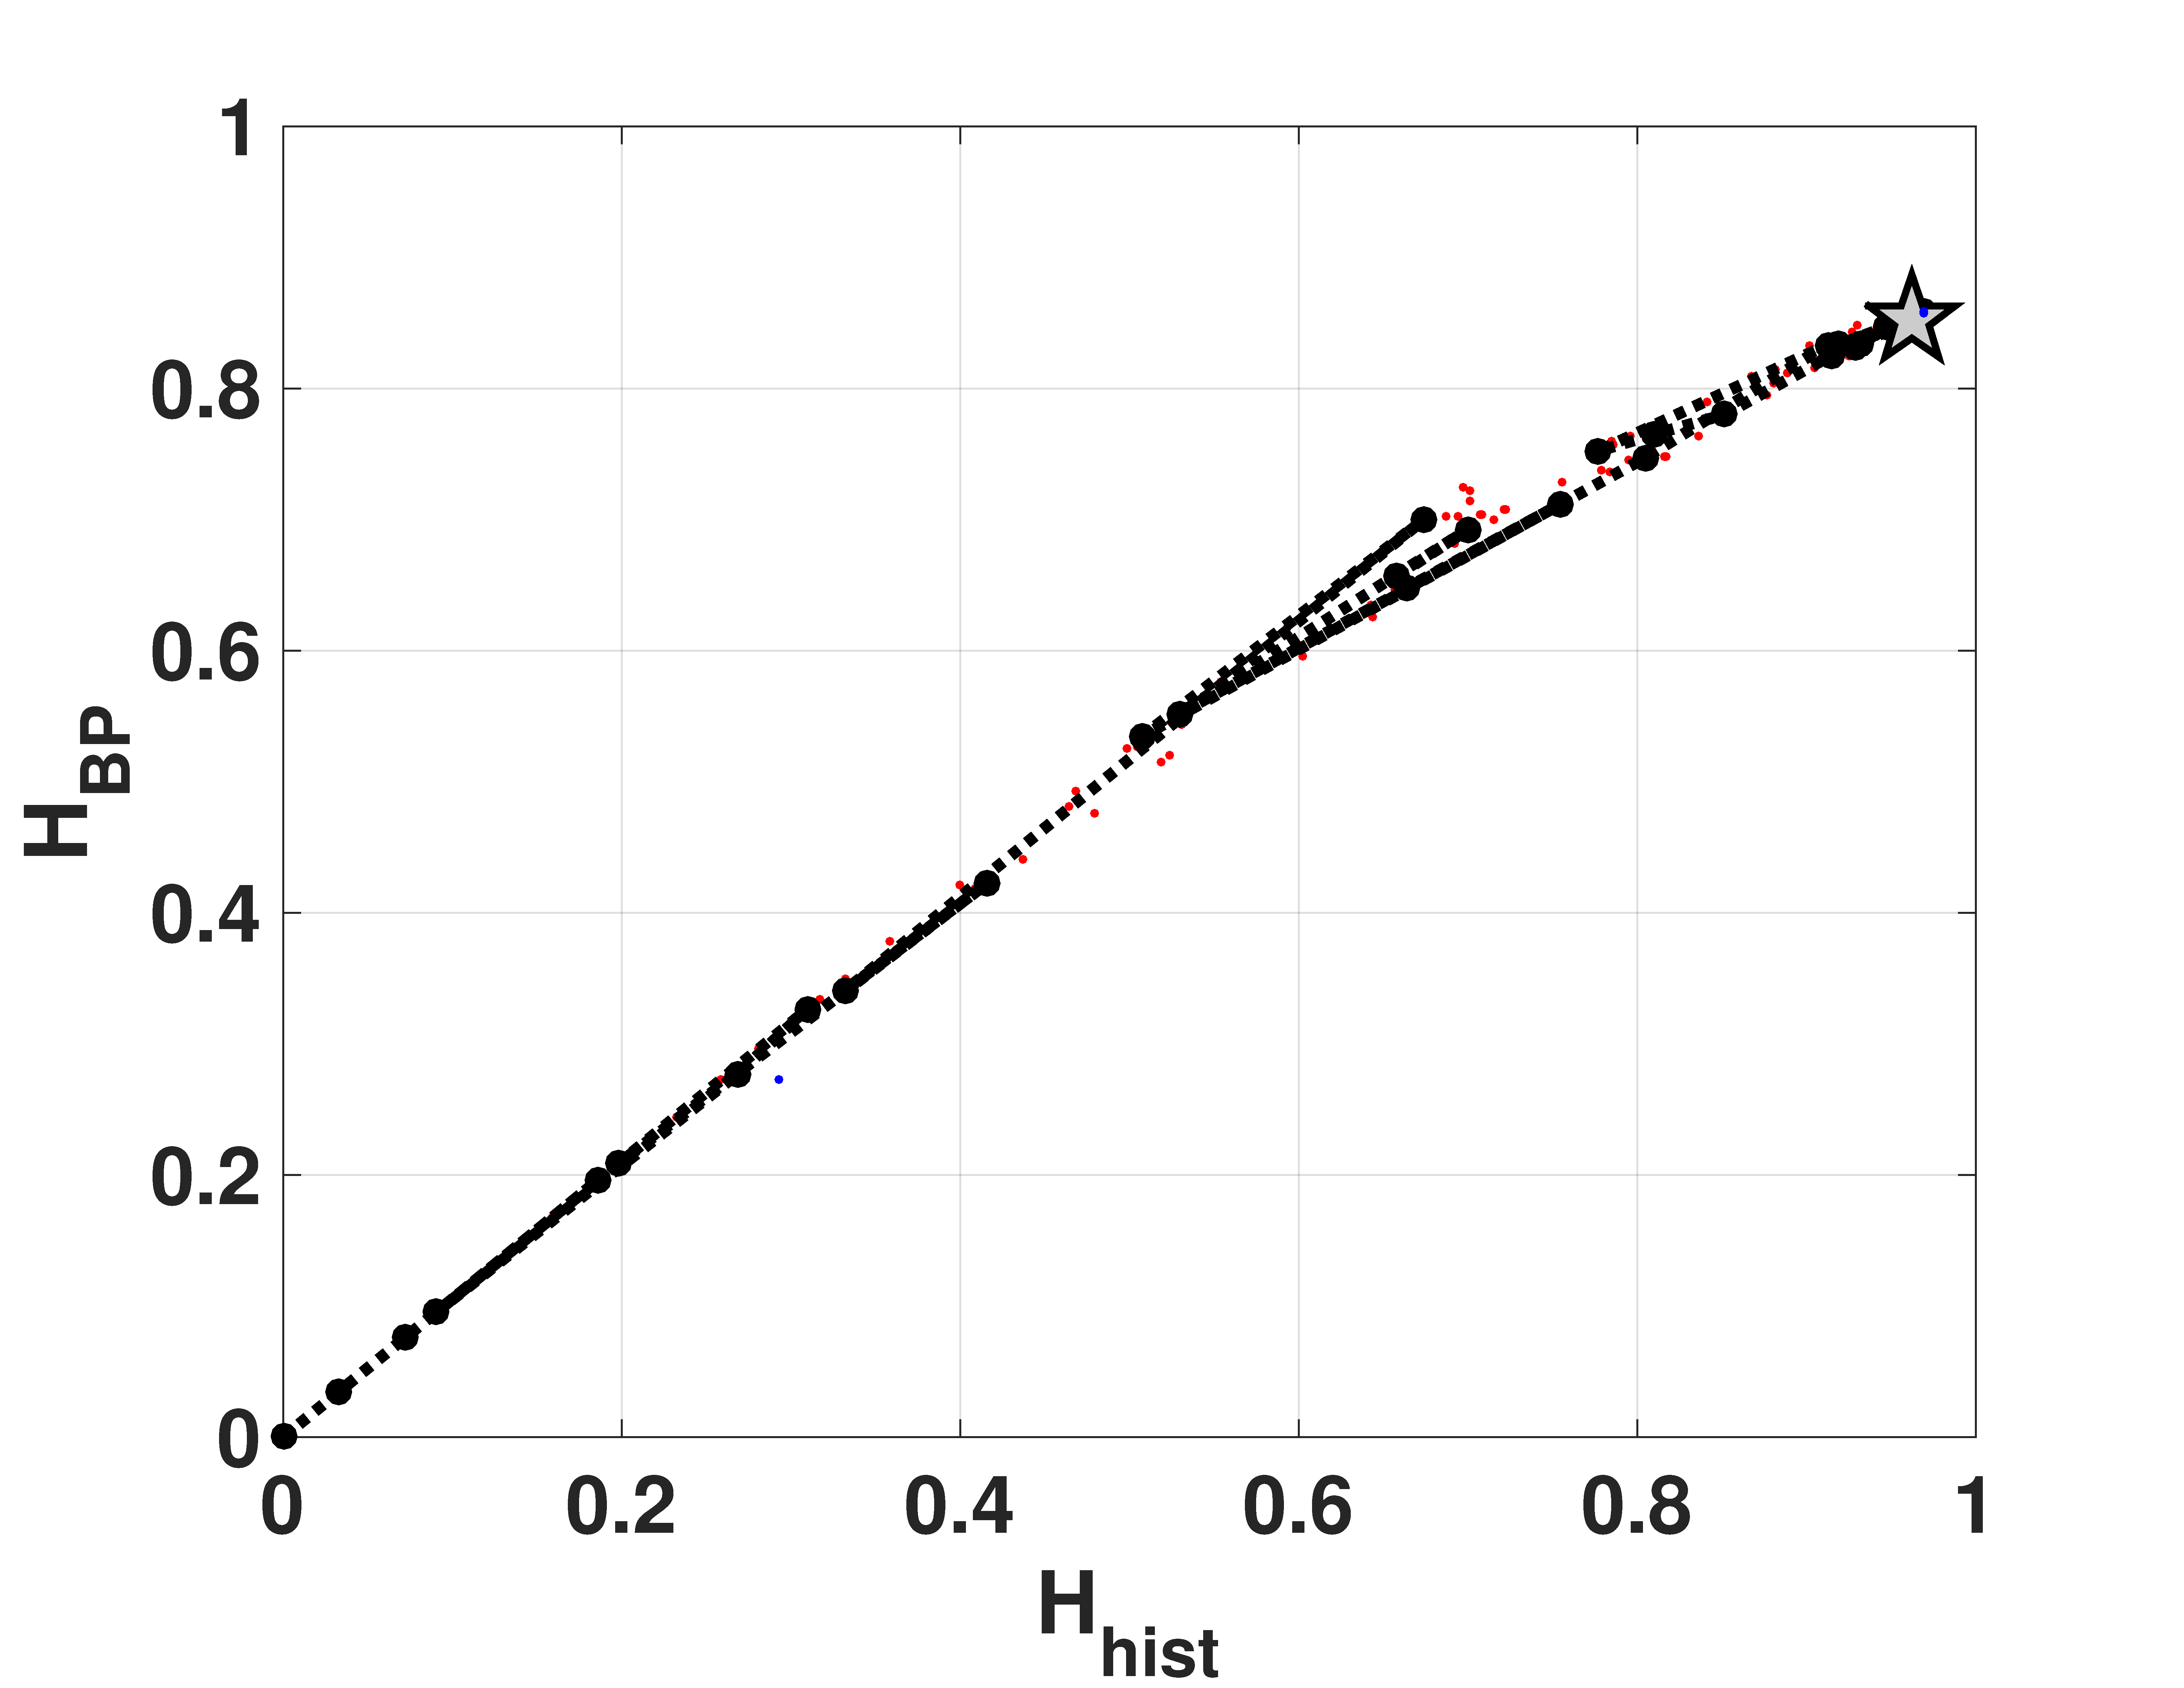
\includegraphics[width=.49\textwidth]{HbpHval_Even}
	\caption{Evolución de las propiedades estadísticas en el plano doble entropía para el mapa EVEN $H_{hist} \times H_{BP}$.}
	\label{fig:EVEN_HH}
\end{figure}
%
\begin{figure}[htpb]
	\centering
	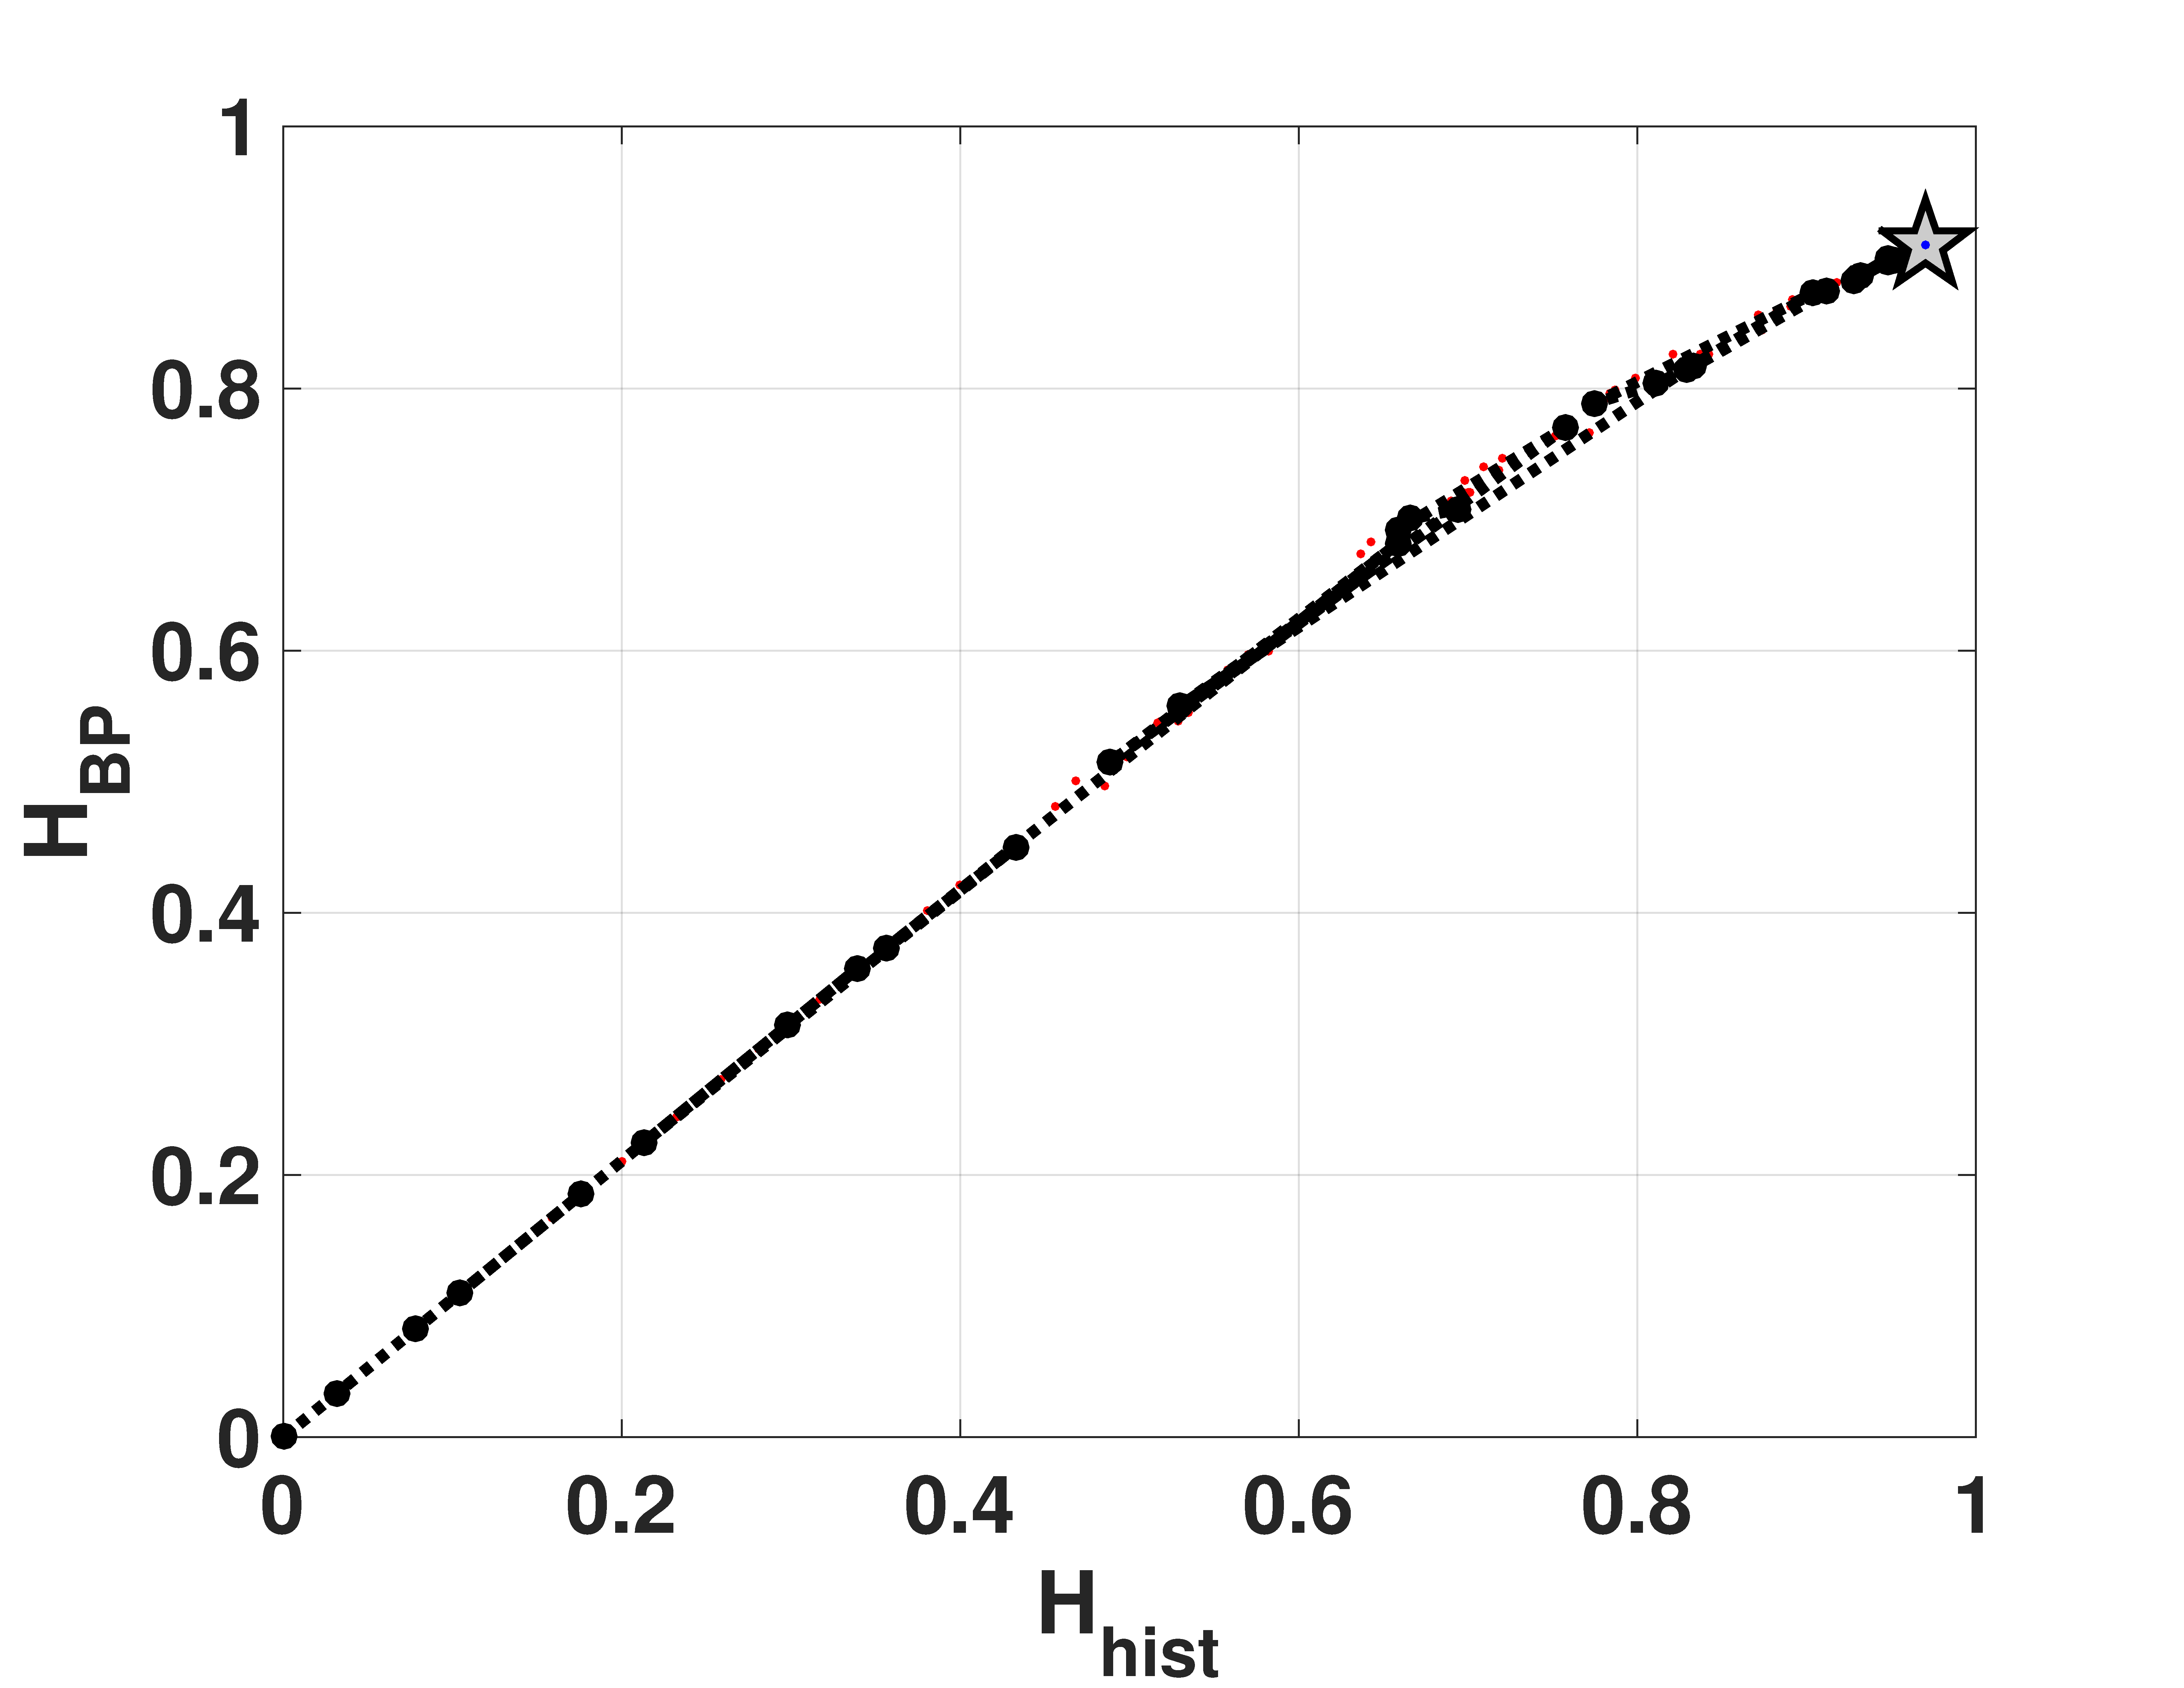
\includegraphics[width=.49\textwidth]{HbpHval_Odd}
	\caption{Evolución de las propiedades estadísticas en el plano doble entropía para el mapa ODD $H_{hist} \times H_{BP}$.}
	\label{fig:ODD_HH}
\end{figure}

Los resultados que se muestran en las Figs. \ref{fig:EVEN_HC} y \ref{fig:ODD_HC} son compatibles, la posición del punto asintótico es más cercana al punto ideal $(H_{hist}, H_{BP}) = (1, 0)$.
Este resultado refleja que la mezcla es mejor porque la complejidad del sistema resultante es menor.
Este plano detecta que en los vectores generados por skipping, la mezcla de ODD es levemente mejor que EVEN.

Compatible results are shown in Figs. \ref{fig:EVEN_HC} and \ref{fig:ODD_HC}, the position of asymptotic point is closest to the ideal point $(H_{hist}, H_{BP})=(1, 0)$.
This result reflects that mixing is better because the complexity of resulting system is lower.
This plane detects that the vector generated by ODD skipping is more mixed than EVEN.
%
\begin{figure}[htpb]
	\centering
	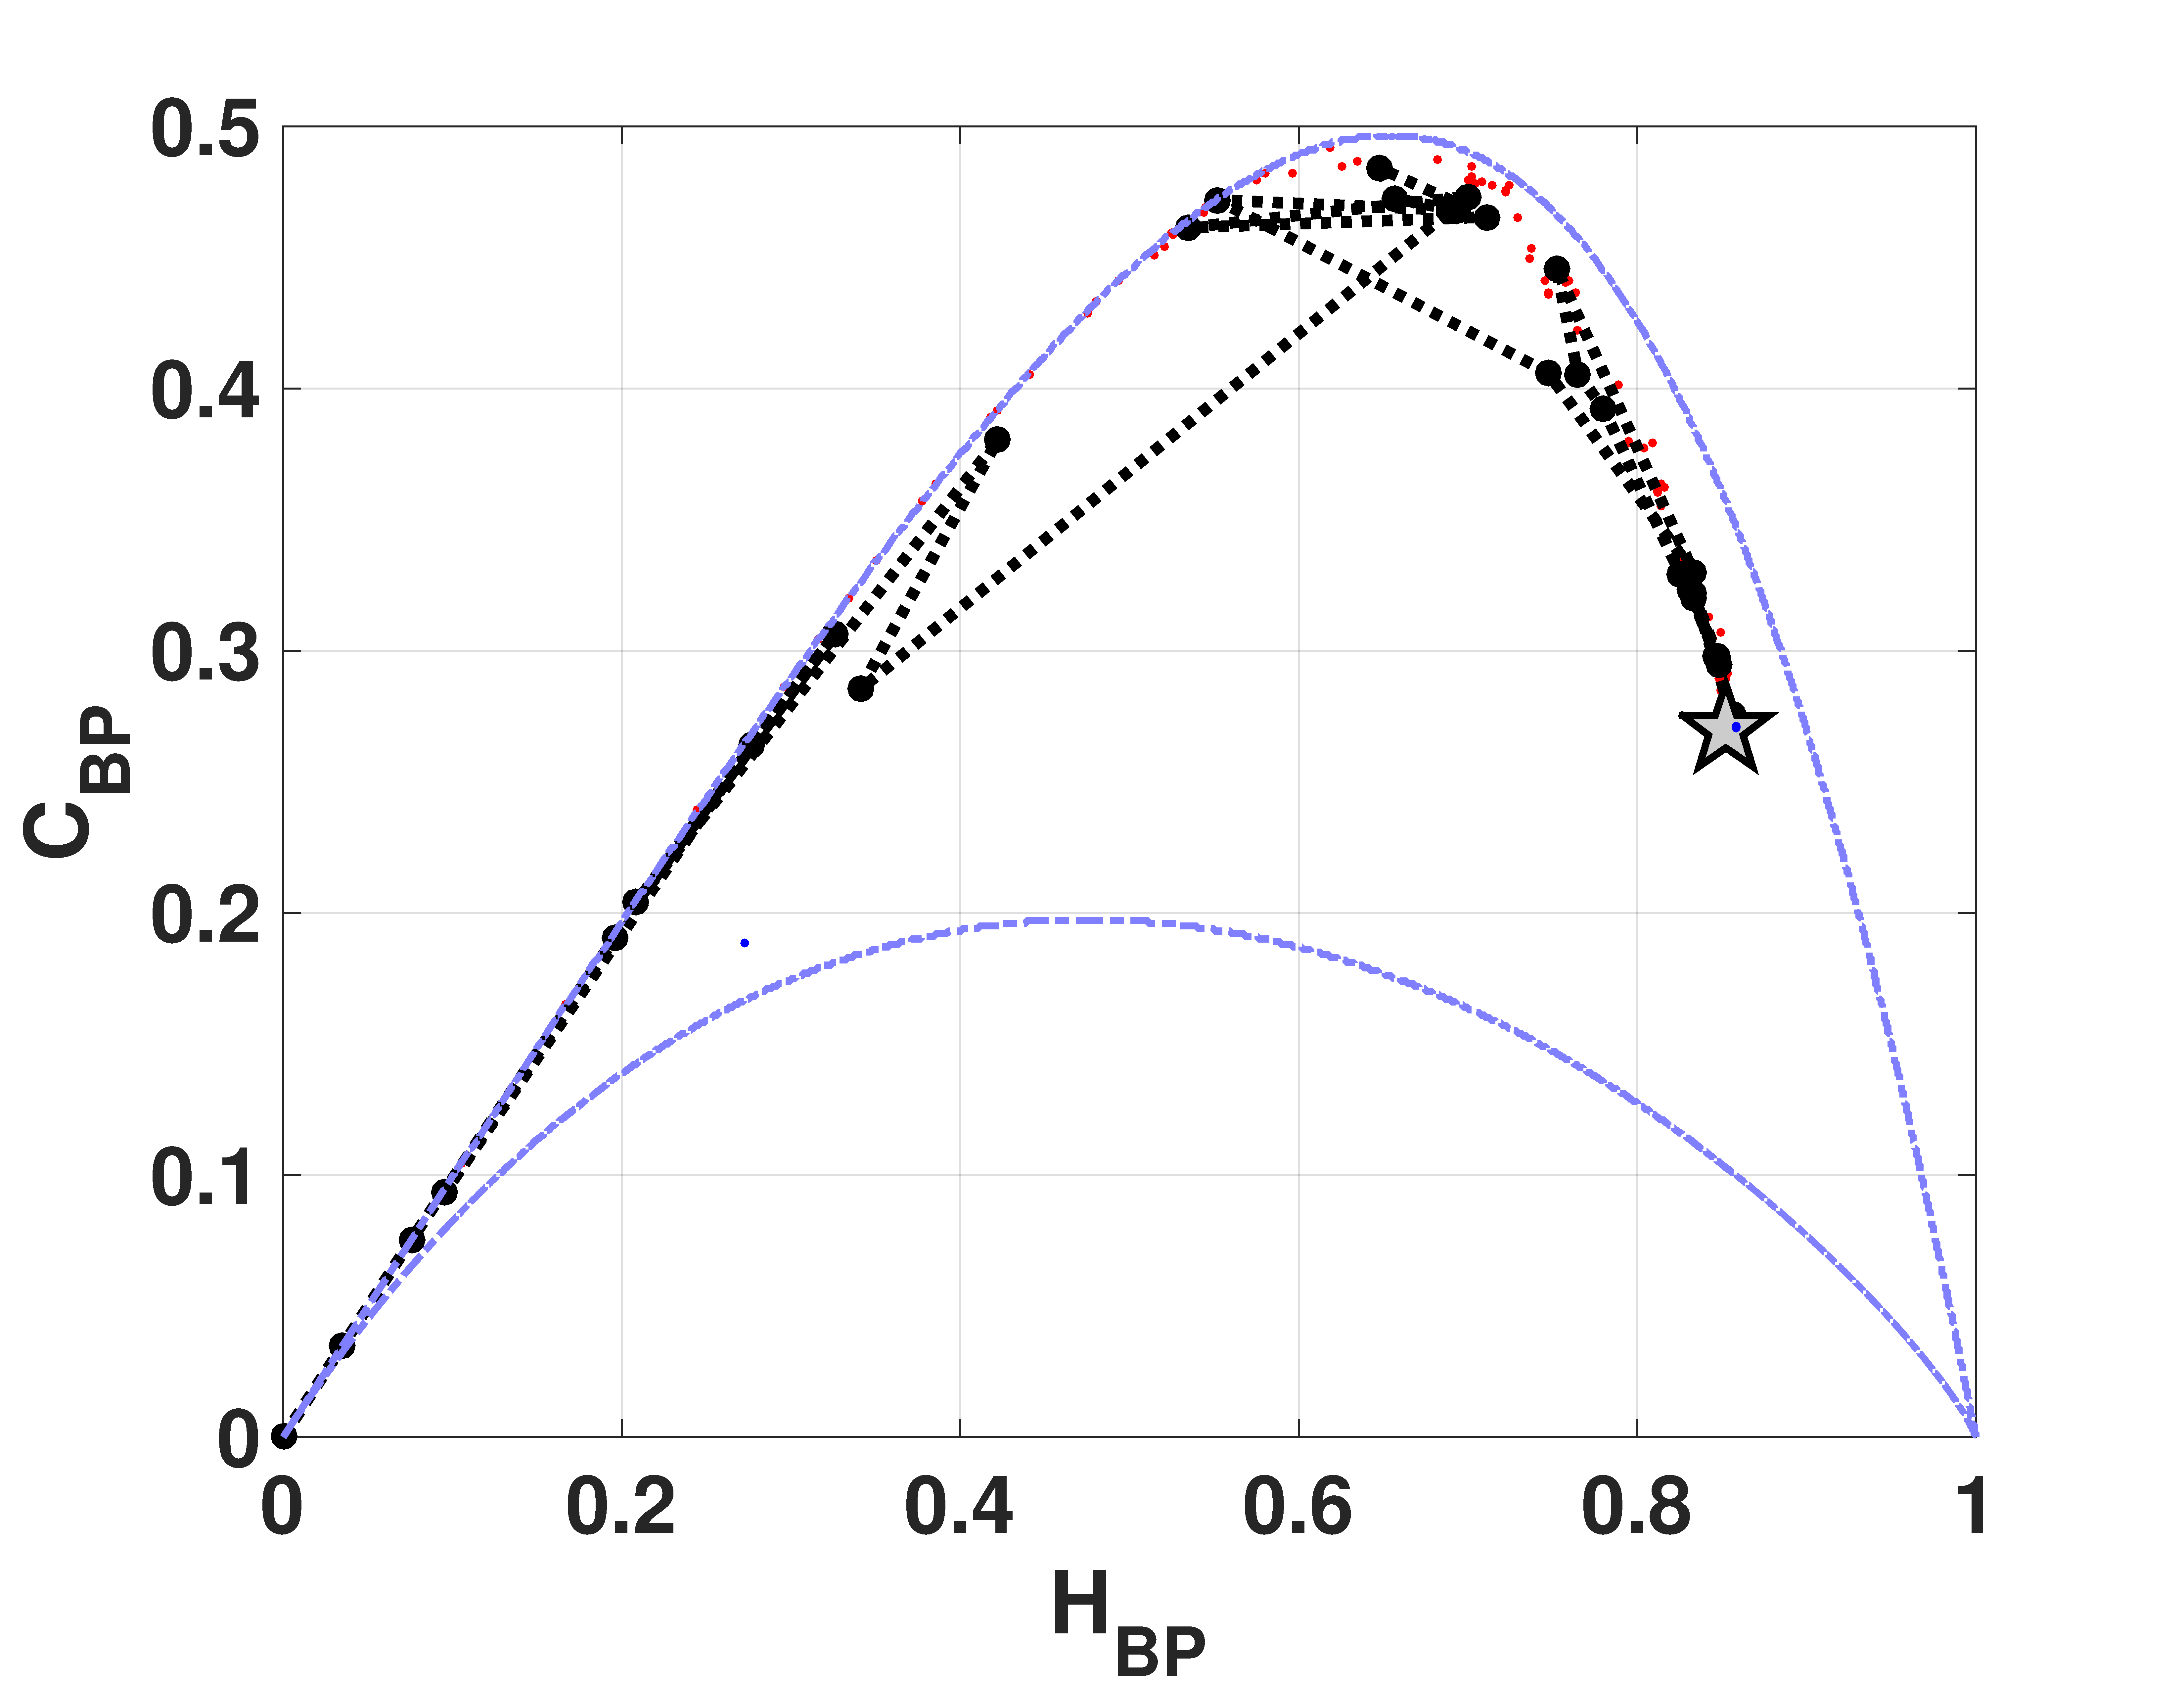
\includegraphics[width=.49\textwidth]{CbpHbp_Even}
	\caption{Evolución de las propiedades estadísticas en el plano entropía - complejidad para el mapa EVEN $H_{BP} \times C_{BP}$.}
	\label{fig:EVEN_HC}
\end{figure}

\begin{figure}[htpb]
	\centering
	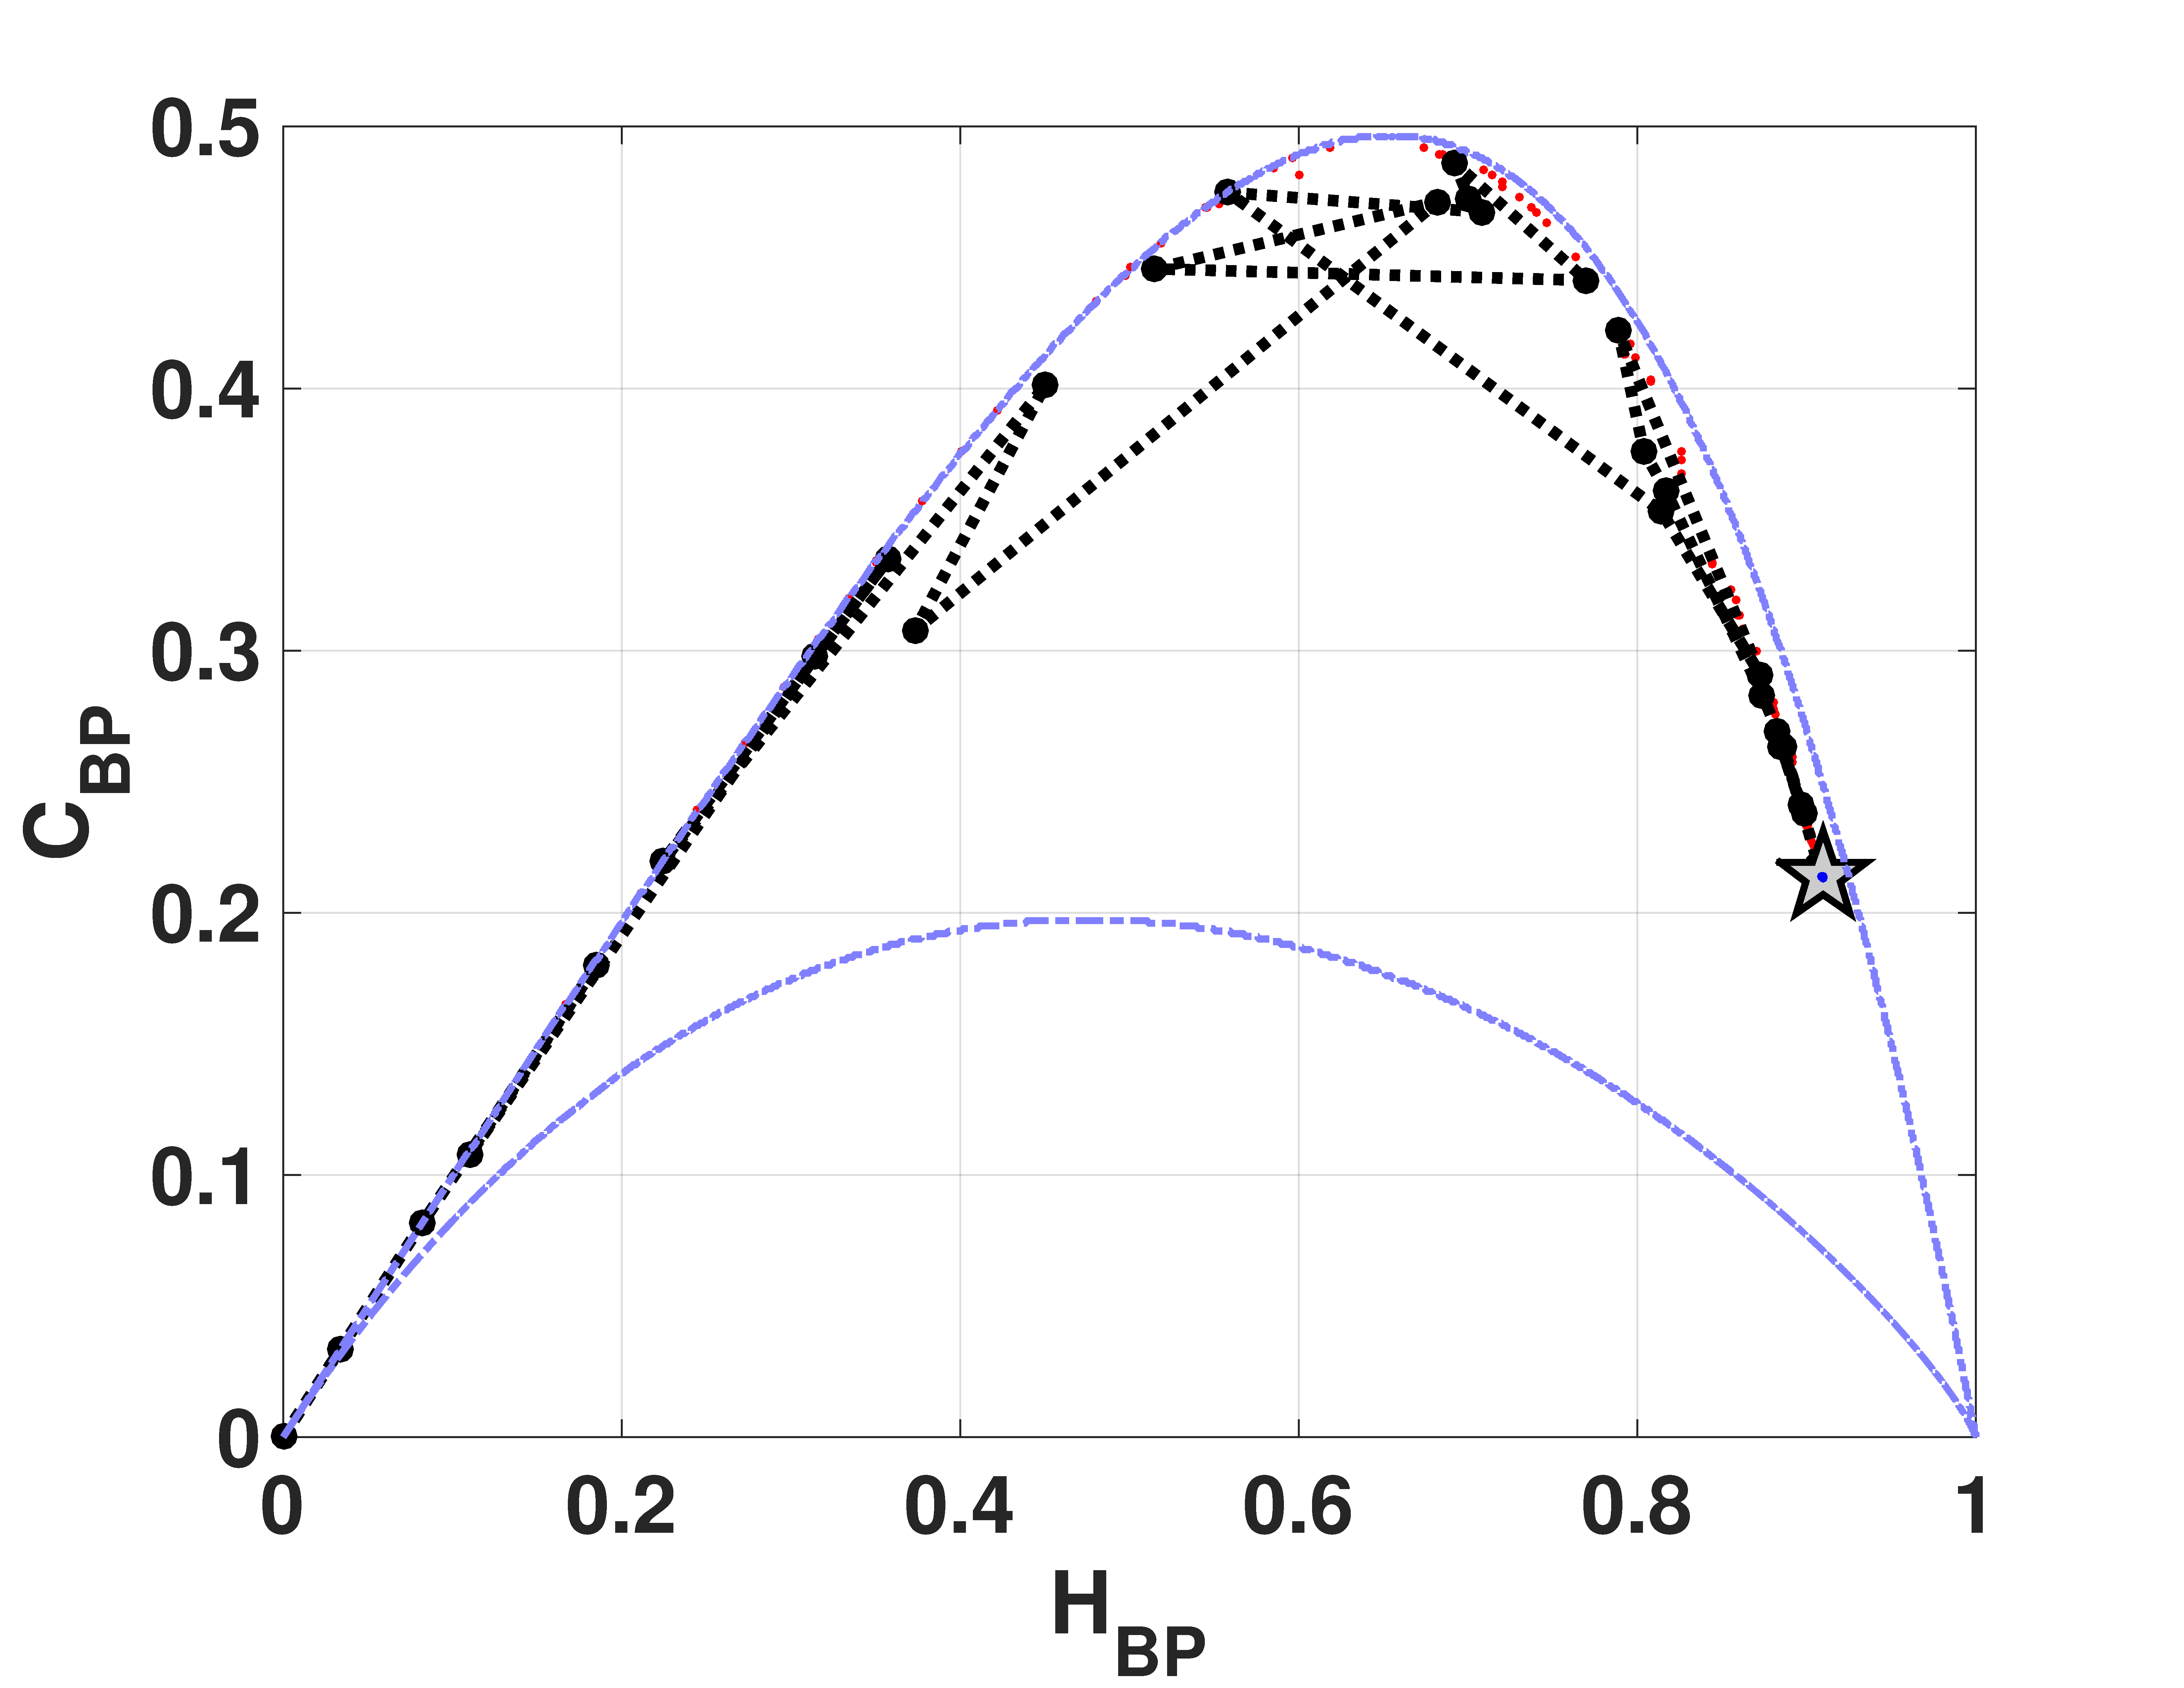
\includegraphics[width=.49\textwidth]{CbpHbp_Odd}
	\caption{Evolución de las propiedades estadísticas en el plano entropía - complejidad para el mapa ODD $H_{BP} \times C_{BP}$.}
	\label{fig:ODD_HC}
\end{figure}